% Aberdeen style guide should be followed when using this
% layout. Their template powerpoint slide is used to extract the
% Aberdeen color and logo but is otherwise ignored (it has little or
% no formatting in it anyway).
%
% http://www.abdn.ac.uk/documents/style-guide.pdf

%%%%%%%%%%%%%%%%%%%% Document Class Settings %%%%%%%%%%%%%%%%%%%%%%%%%
% Pick if you want slides, or draft slides (no animations)
%%%%%%%%%%%%%%%%%%%%%%%%%%%%%%%%%%%%%%%%%%%%%%%%%%%%%%%%%%%%%%%%%%%%%%
%Normal document mode
\documentclass[10pt,compress, unknownkeysallowed]{beamer}
%Draft or handout mode
%\documentclass[10pt,compress,handout]{beamer}
%\documentclass[10pt,compress,handout,ignorenonframetext]{beamer} 
\usepackage{xcolor}

\newlength{\overwritelength}
\newlength{\minimumoverwritelength}
\setlength{\minimumoverwritelength}{1cm}
\newcommand{\overwrite}[3][red]{%
  \settowidth{\overwritelength}{$#2$}%
  \ifdim\overwritelength<\minimumoverwritelength%
    \setlength{\overwritelength}{\minimumoverwritelength}\fi%
  \stackrel
    {%
      \begin{minipage}{\overwritelength}%
        \color{#1}\centering\small #3\\%
        \rule{1pt}{9pt}%
      \end{minipage}}
    {\colorbox{#1!50}{\color{black}$\displaystyle#2$}}}


%%%%%%%%%%%%%%%%%%%% General Document settings %%%%%%%%%%%%%%%%%%%%%%%
% These settings must be set for each presentation
%%%%%%%%%%%%%%%%%%%%%%%%%%%%%%%%%%%%%%%%%%%%%%%%%%%%%%%%%%%%%%%%%%%%%%
\newcommand{\shortname}{} 
\newcommand{\fullname}{}
\institute{School of Engineering}
\newcommand{\emailaddress}{}%{jefferson.gomes@abdn.ac.uk}
\subtitle{Brief Overview of CFD Workflow: Modelling Laminar Pipe Flow using ANSYS Fluent}
\newcommand{\logoimage}{./FigBanner/UoAHorizBanner}
\title{Computational Fluid Dynamics (EG501V)}
%\subtitle{Introduction to CFD Practice}
\date[]{}


%%%%%%%%%%%%%%%%%%%% Template settings %%%%%%%%%%%%%%%%%%%%%%%%%%%%%%%
% You shouldn't have to change below this line, unless you want to.
%%%%%%%%%%%%%%%%%%%%%%%%%%%%%%%%%%%%%%%%%%%%%%%%%%%%%%%%%%%%%%%%%%%%%%
\usecolortheme{whale}
\useoutertheme{infolines}

% Use the fading effect for items that are covered on the current
% slide.
\beamertemplatetransparentcovered

% We abuse the author command to place all of the slide information on
% the title page.
\author[\shortname]{%
  \fullname\\\ttfamily{\emailaddress}
}


%At the start of every section, put a slide indicating the contents of the current section.
\AtBeginSection[] {
  \begin{frame}
    \frametitle{Section Outline}
    \tableofcontents[currentsection]
  \end{frame}
}

% Allow the inclusion of movies into the Presentation! At present,
% only the Okular program is capable of playing the movies *IN* the
% presentation.
\usepackage{multimedia}
\usepackage{animate}

%% Handsout -- comment out the lines below to create handstout with 4 slides in a page with space for comments
\usepackage{handoutWithNotes}

\mode<handout>
{
\usepackage{pgf,pgfpages}

\pgfpagesdeclarelayout{2 on 1 boxed with notes}
{
\edef\pgfpageoptionheight{\the\paperheight} 
\edef\pgfpageoptionwidth{\the\paperwidth}
\edef\pgfpageoptionborder{0pt}
}
{
\setkeys{pgfpagesuselayoutoption}{landscape}
\pgfpagesphysicalpageoptions
    {%
        logical pages=4,%
        physical height=\pgfpageoptionheight,%
        physical width=\pgfpageoptionwidth,%
        last logical shipout=2%
    } 
\pgfpageslogicalpageoptions{1}
    {%
    border code=\pgfsetlinewidth{1pt}\pgfstroke,%
    scale=1,
    center=\pgfpoint{.25\pgfphysicalwidth}{.75\pgfphysicalheight}%
    }%
\pgfpageslogicalpageoptions{2}
    {%
    border code=\pgfsetlinewidth{1pt}\pgfstroke,%
    scale=1,
    center=\pgfpoint{.25\pgfphysicalwidth}{.25\pgfphysicalheight}%
    }%
\pgfpageslogicalpageoptions{3}
    {%
    border shrink=\pgfpageoptionborder,%
    resized width=.7\pgfphysicalwidth,%
    resized height=.5\pgfphysicalheight,%
    center=\pgfpoint{.75\pgfphysicalwidth}{.29\pgfphysicalheight},%
    copy from=3
    }%
\pgfpageslogicalpageoptions{4}
    {%
    border shrink=\pgfpageoptionborder,%
    resized width=.7\pgfphysicalwidth,%
    resized height=.5\pgfphysicalheight,%
    center=\pgfpoint{.75\pgfphysicalwidth}{.79\pgfphysicalheight},%
    copy from=4
    }%

\AtBeginDocument
    {
    \newbox\notesbox
    \setbox\notesbox=\vbox
        {
            \hsize=\paperwidth
            \vskip-1in\hskip-1in\vbox
            {
                \vskip1cm
                Notes\vskip1cm
                        \hrule width\paperwidth\vskip1cm
                    \hrule width\paperwidth\vskip1cm
                        \hrule width\paperwidth\vskip1cm
                    \hrule width\paperwidth\vskip1cm
                        \hrule width\paperwidth\vskip1cm
                    \hrule width\paperwidth\vskip1cm
                    \hrule width\paperwidth\vskip1cm
                    \hrule width\paperwidth\vskip1cm
                        \hrule width\paperwidth
            }
        }
        \pgfpagesshipoutlogicalpage{3}\copy\notesbox
        \pgfpagesshipoutlogicalpage{4}\copy\notesbox
    }
}
}

%\pgfpagesuselayout{2 on 1 boxed with notes}[letterpaper,border shrink=5mm]
%\pgfpagesuselayout{2 on 1 boxed with notes}[letterpaper,border shrink=5mm]

%%%%% Color settings
\usepackage{color}
%% The background color for code listings (i.e. example programs)
\definecolor{lbcolor}{rgb}{0.9,0.9,0.9}%
\definecolor{UoARed}{rgb}{0.64706, 0.0, 0.12941}
\definecolor{UoALight}{rgb}{0.85, 0.85, 0.85}
\definecolor{UoALighter}{rgb}{0.92, 0.92, 0.92}
\setbeamercolor{structure}{fg=UoARed} % General background and higlight color
\setbeamercolor{frametitle}{bg=black} % General color
\setbeamercolor{frametitle right}{bg=black} % General color
\setbeamercolor{block body}{bg=UoALighter} % For blocks
\setbeamercolor{structure}{bg=UoALight} % For blocks
% Rounded boxes for blocks
\setbeamertemplate{blocks}[rounded]

%%%%% Font settings
% Aberdeen requires the use of Arial in slides. We can use the
% Helvetica font as its widely available like so
% \usepackage{helvet}
% \renewcommand{\familydefault}{\sfdefault}
% But beamer already uses a sans font, so we will stick with that.

% The size of the font used for the code listings.
\newcommand{\goodsize}{\fontsize{6}{7}\selectfont}

% Extra math packages, symbols and colors. If you're using Latex you
% must be using it for formatting the math!
\usepackage{amscd,amssymb} \usepackage{amsfonts}
\usepackage[mathscr]{eucal} \usepackage{mathrsfs}
\usepackage{latexsym} \usepackage{amsmath} \usepackage{bm}
\usepackage{amsthm} \usepackage{textcomp} \usepackage{eurosym}
% This package provides \cancel{a} and \cancelto{a}{b} to "cancel"
% expressions in math.
\usepackage{cancel}

\usepackage{comment} 

% Get rid of font warnings as modern LaTaX installations have scalable
% fonts
\usepackage{type1cm} 

%\usepackage{enumitem} % continuous numbering throughout enumerate commands

% For exact placement of images/text on the cover page
\usepackage[absolute]{textpos}
\setlength{\TPHorizModule}{1mm}%sets the textpos unit
\setlength{\TPVertModule}{\TPHorizModule} 

% Source code formatting package
\usepackage{listings}%
\lstset{ backgroundcolor=\color{lbcolor}, tabsize=4,
  numberstyle=\tiny, rulecolor=, language=C++, basicstyle=\goodsize,
  upquote=true, aboveskip={1.5\baselineskip}, columns=fixed,
  showstringspaces=false, extendedchars=true, breaklines=false,
  prebreak = \raisebox{0ex}[0ex][0ex]{\ensuremath{\hookleftarrow}},
  frame=single, showtabs=false, showspaces=false,
  showstringspaces=false, identifierstyle=\ttfamily,
  keywordstyle=\color[rgb]{0,0,1},
  commentstyle=\color[rgb]{0.133,0.545,0.133},
  stringstyle=\color[rgb]{0.627,0.126,0.941}}

% Allows the inclusion of other PDF's into the final PDF. Great for
% attaching tutorial sheets etc.
\usepackage{pdfpages}
\setbeamercolor{background canvas}{bg=}  

% Remove foot note horizontal rules, they occupy too much space on the slide
\renewcommand{\footnoterule}{}

% Force the driver to fix the colors on PDF's which include mixed
% colorspaces and transparency.
\pdfpageattr {/Group << /S /Transparency /I true /CS /DeviceRGB>>}

% Include a graphics, reserve space for it but
% show it on the next frame.
% Parameters:
% #1 Which slide you want it on
% #2 Previous slides
% #3 Options to \includegraphics (optional)
% #4 Name of graphic
\newcommand{\reserveandshow}[4]{%
\phantom{\includegraphics<#2|handout:0>[#3]{#4}}%
\includegraphics<#1>[#3]{#4}%
}

\newcommand{\frc}{\displaystyle\frac}
\newcommand{\red}{\textcolor{red}}
\newcommand{\blue}{\textcolor{blue}}
\newcommand{\green}{\textcolor{green}}
\newcommand{\purple}{\textcolor{purple}}
\newcommand{\eg}{{\it e.g., }}
\newcommand{\ie}{{\it i.e., }}
\newcommand{\wrt}{{\it wrt }}
 

\begin{document}

% Title page layout
\begin{frame}
  \titlepage
  \vfill%
  \begin{center}
    \includegraphics[clip,width=0.8\textwidth]{\logoimage}
  \end{center}
\end{frame}

% Table of contents
\frame{ \frametitle{Slides Outline}
  \tableofcontents
}


%%%%%%%%%%%%%%%%%%%% The Presentation Proper %%%%%%%%%%%%%%%%%%%%%%%%%
% Fill below this line with \begin{frame} commands! It's best to
% always add the fragile option incase you're going to use the
% verbatim environment.
%%%%%%%%%%%%%%%%%%%%%%%%%%%%%%%%%%%%%%%%%%%%%%%%%%%%%%%%%%%%%%%%%%%%%%



%##################
%%%  SECTION
%##################
\section{Motivation}
%%%
%%% Slide
%%%
\begin{frame}
 \frametitle{Initial Definition}

\begin{enumerate}
\item <1->\textcolor{blue}{Computational Fluid Dynamics (CFD)} is a numerical tool to predict (qualitatively and quantitatively) fluid flow using:
\begin{enumerate}
\item <2-> Mathematical modelling $\rightarrow$ representing the physics by partial differential equations (PDE);
\item <3-> Numerical methods $\rightarrow$ set of discretisation and solution techniques for the PDE and;
\item <4-> Software tools $\rightarrow$ set of solvers, pre- and post-processing technologies.
\end{enumerate}
\item <5-> \textcolor{blue}{Numerical simulations} produced by CFD models can be seen as \red{$\lq$Virtual Fluid Flow Laboratory'};
\item <6-> \textcolor{blue}{CFD} is more cost-effective (i.e., less financially expansive) than experimental testing;
\item <7-> \textcolor{blue}{CFD} has been used to:
\begin{enumerate}
\item <8-> Improve the understanding of the fluid flow and potential interactions with solids (e.g., internal structures), chemical reactions, etc;
\item <9-> Assess the performance of equipment / facilities;
\item <10-> Aid in the design of new equipment / facilities;
\item <11-> Identify potential operational problems (e.g., safety and environmental assessment of industrial processes);
\item <12-> Guide experiments.
\end{enumerate}

\end{enumerate}
 
\end{frame}

%%%
%%% Slide
%%%
\begin{frame}
 \frametitle{Motivation: Environmental and Industrial Flows}

   \begin{figure}%
    \begin{center}
     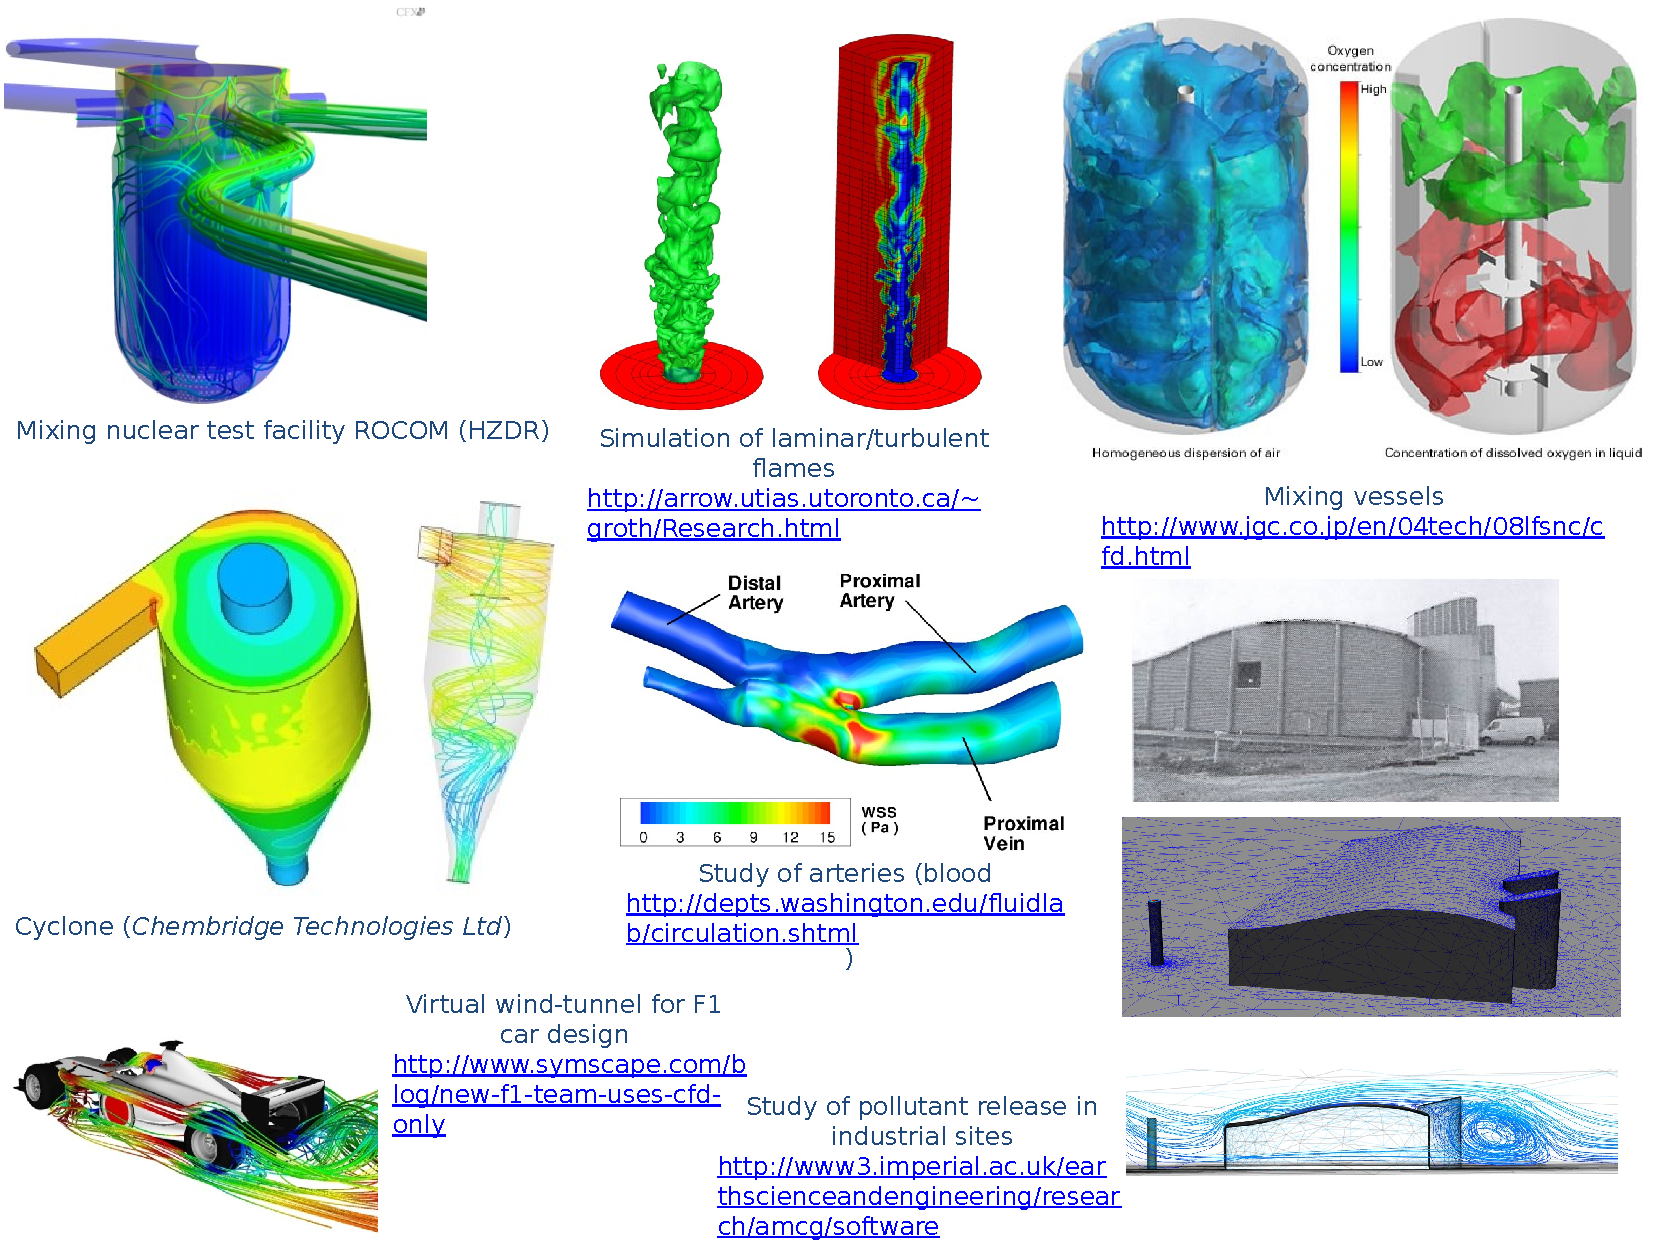
\includegraphics[width=12.cm, height=7.8cm, clip]{./Figs/SpecificIndustrialEnvironmentalApplication2}
    \end{center}
%\caption{XX}
   \end{figure}    
\end{frame}
 
%%%
%%% Slide
%%%
\begin{frame}
 \frametitle{Motivation: Environmental and Industrial Flows}

   \begin{figure}%
    \begin{center}
     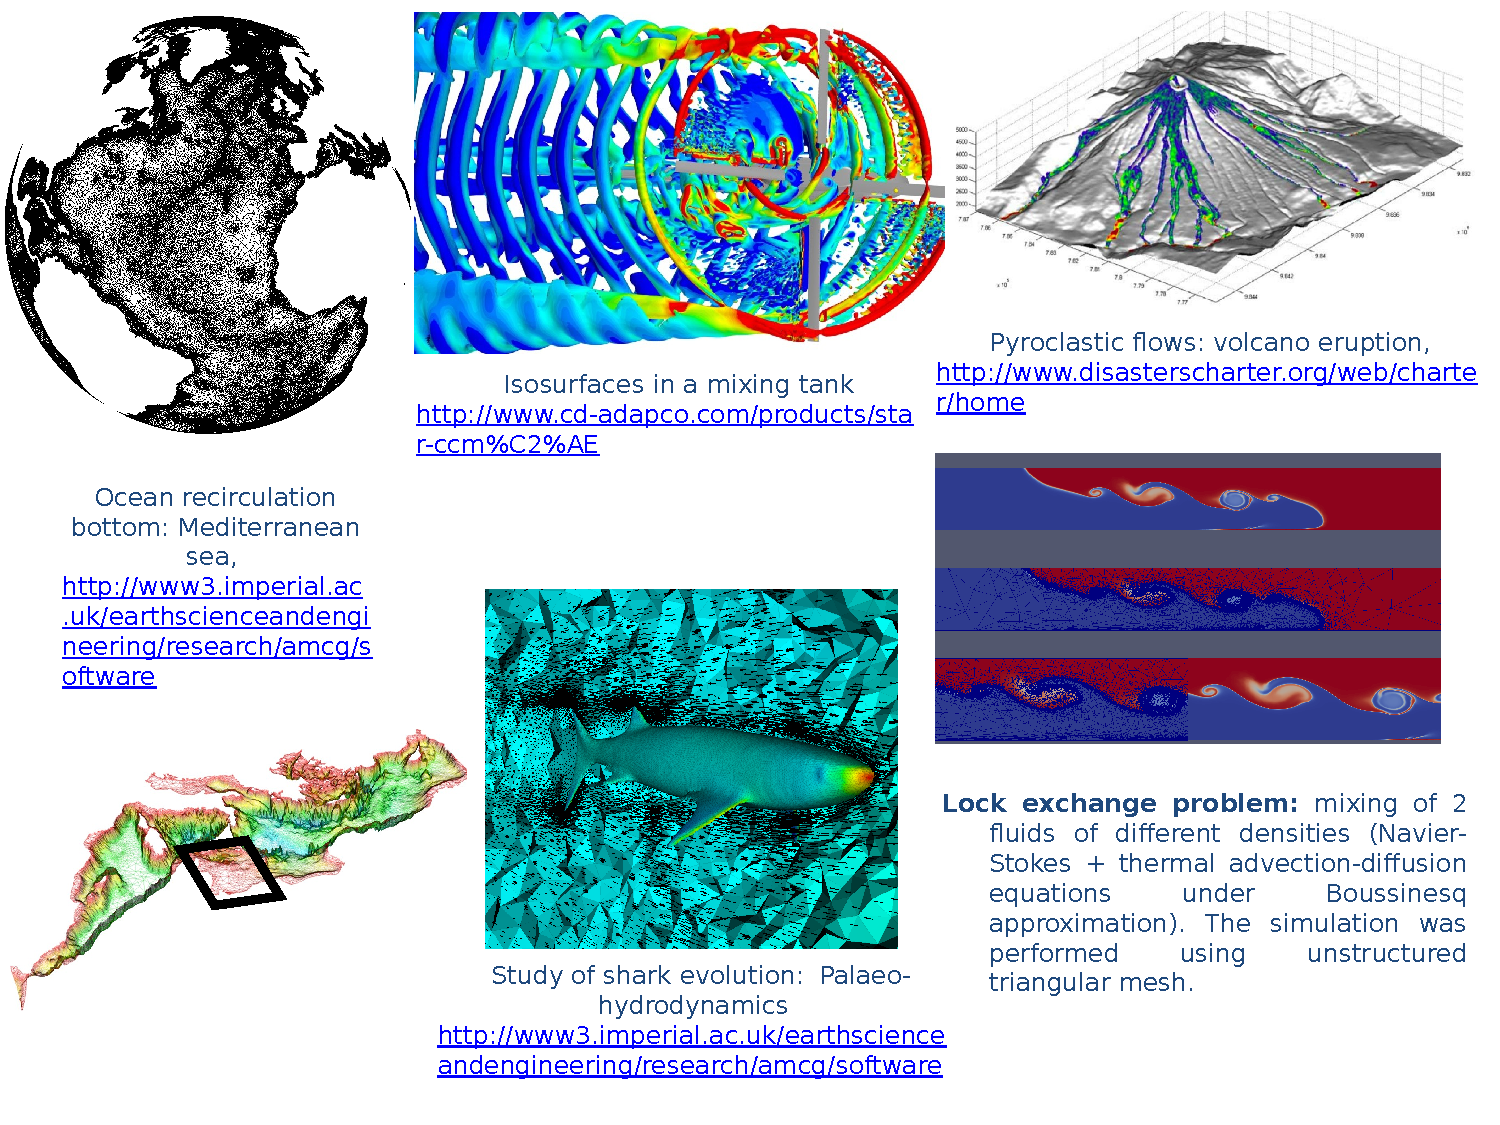
\includegraphics[width=12.cm, height=7.8cm, clip]{./Figs/PostProcessingExamples2.pdf}
    \end{center}
%\caption{XX}
   \end{figure}    
\end{frame}

%%%
%%% Slide
%%%
\begin{frame}
 \frametitle{Field Observation, Experiments and Numerical Simulations} 

   \begin{figure}%
    \begin{center}
     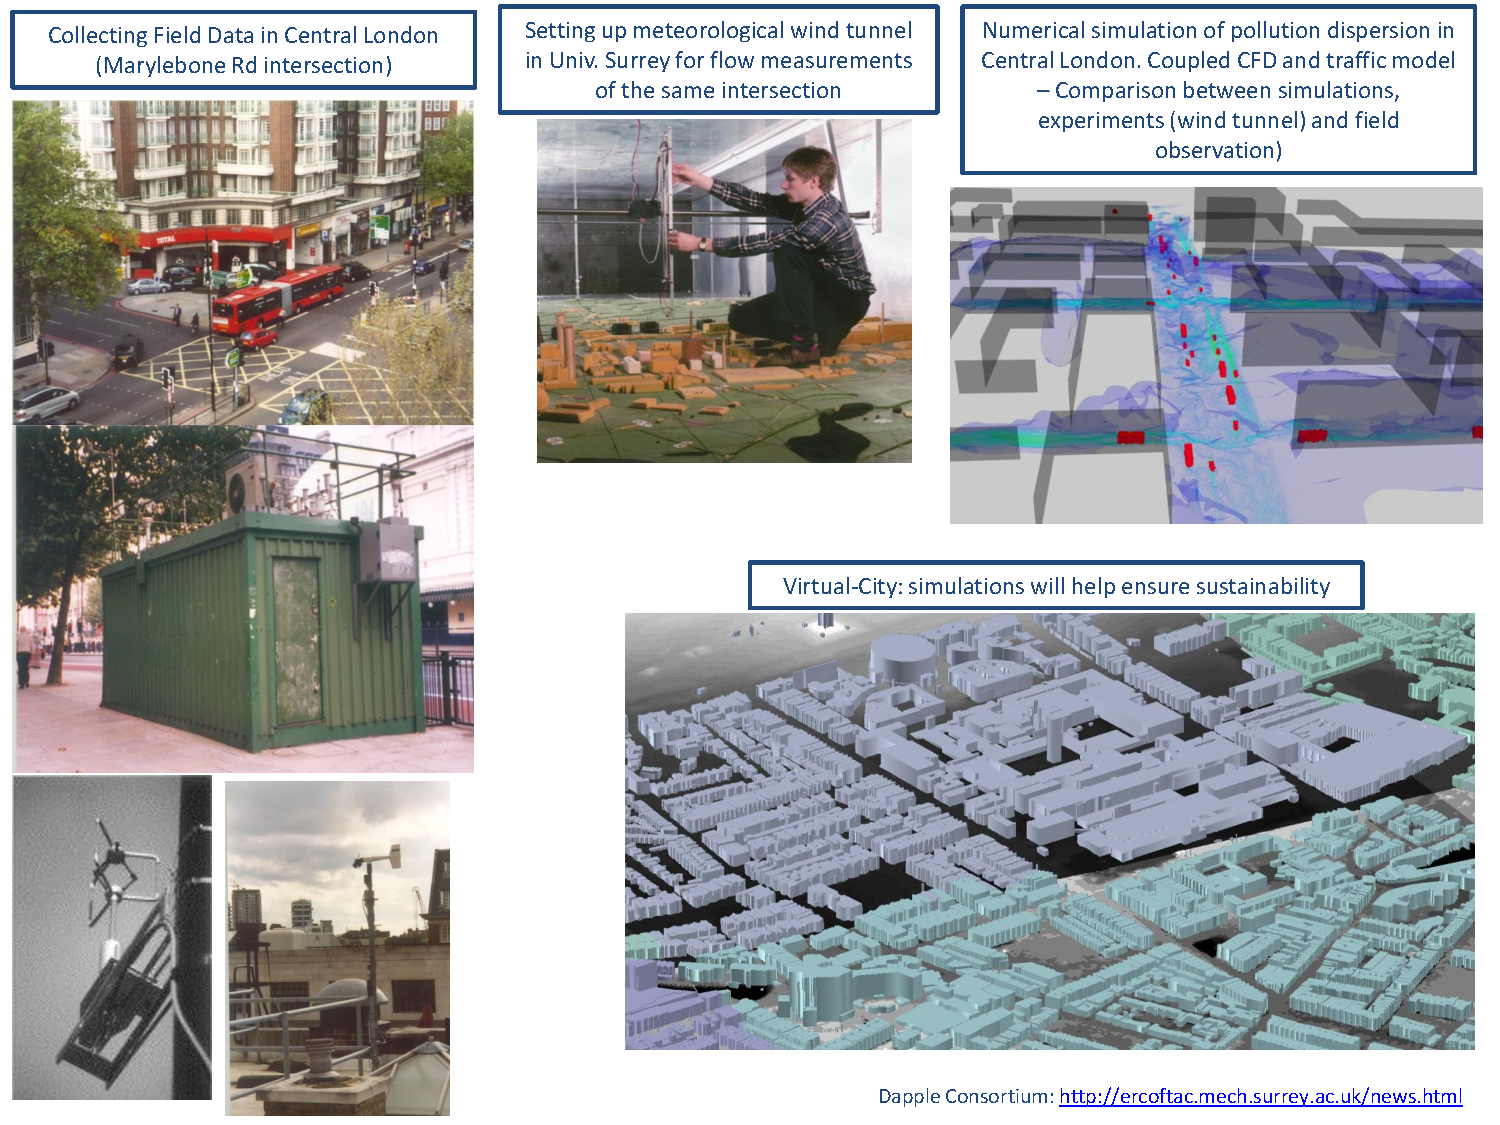
\includegraphics[width=12.cm, height=7.8cm, clip]{./Figs/Dapple.pdf}
    \end{center}
%\caption{XX}
   \end{figure}    
\end{frame}
%%%
%%% Slide
%%%
\begin{frame}
 \frametitle{Example: Pollution dispersion in an industrial site}

   \begin{figure}%
    \begin{center}
     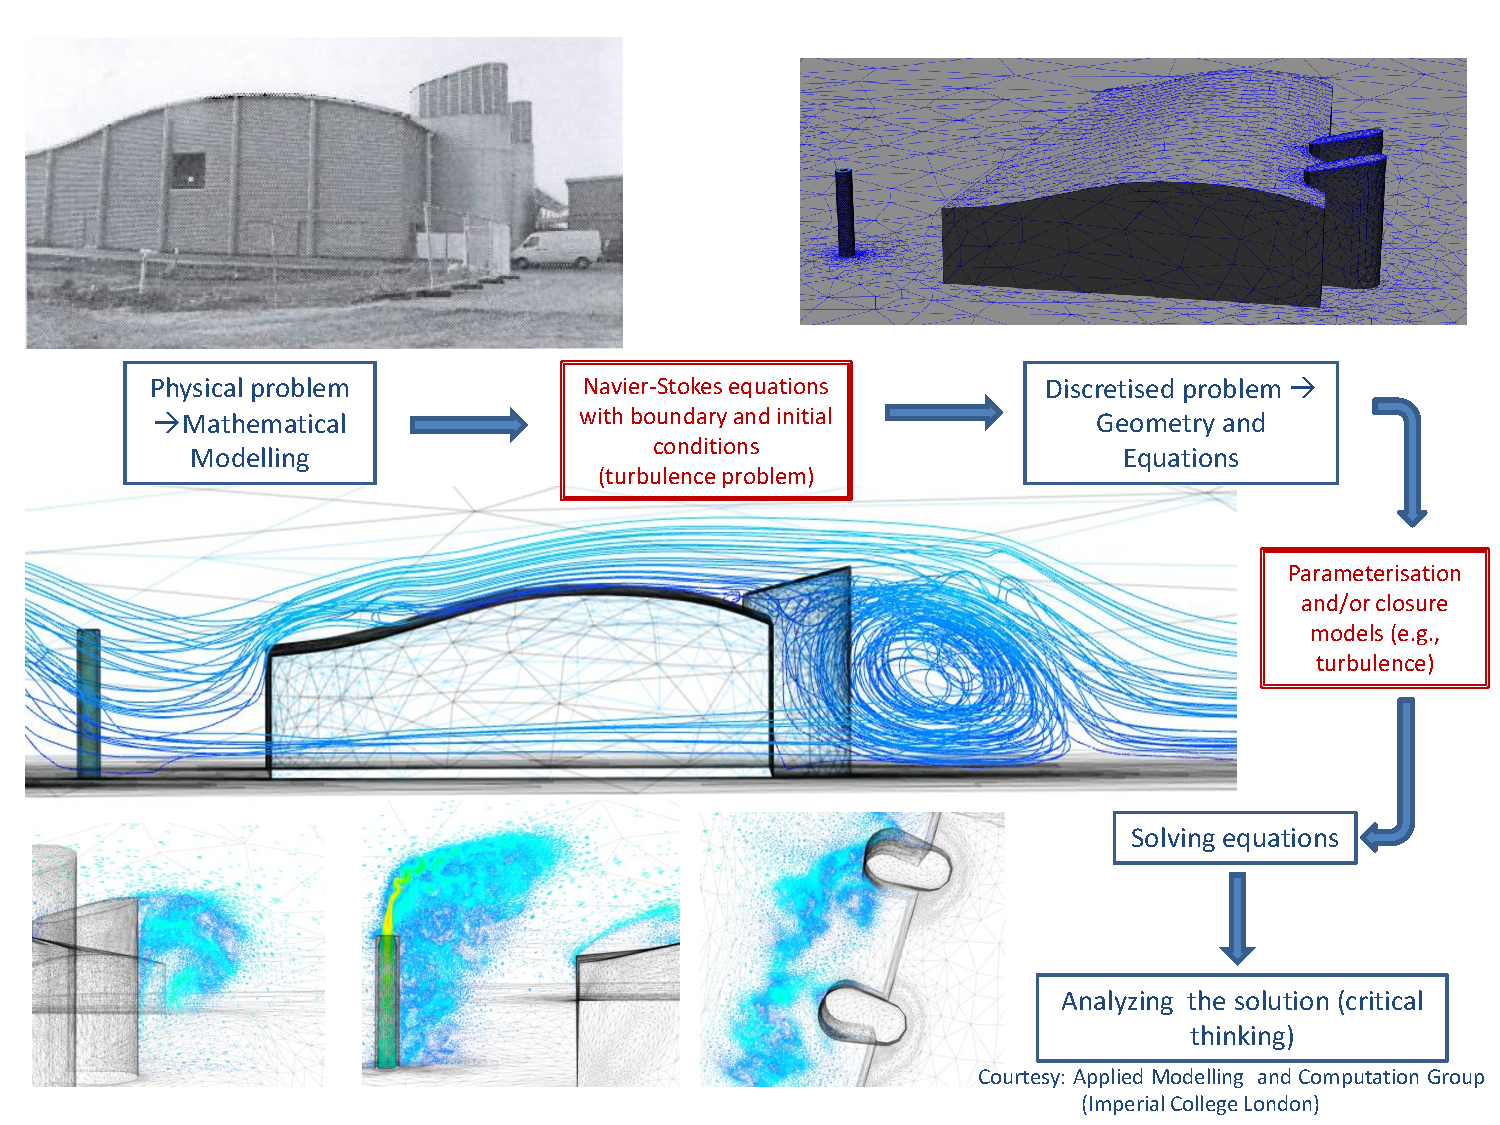
\includegraphics[width=12.cm, height=7.8cm, clip]{./Figs/SpecificIndustrialEnvironmentalApplication.pdf}
    \end{center}
%\caption{XX}
   \end{figure}    

\end{frame}


%%%%%%%%%%%%%%%%%%%
%%%   SECTION   %%%
%%%%%%%%%%%%%%%%%%%
\section{Workflow for Computational Fluid Dynamics (CFD) Simulations}

%%%
%%% Slide
%%%
\begin{frame}
 \frametitle{Overview: Workflow}

   \begin{figure}%
    \begin{center}
     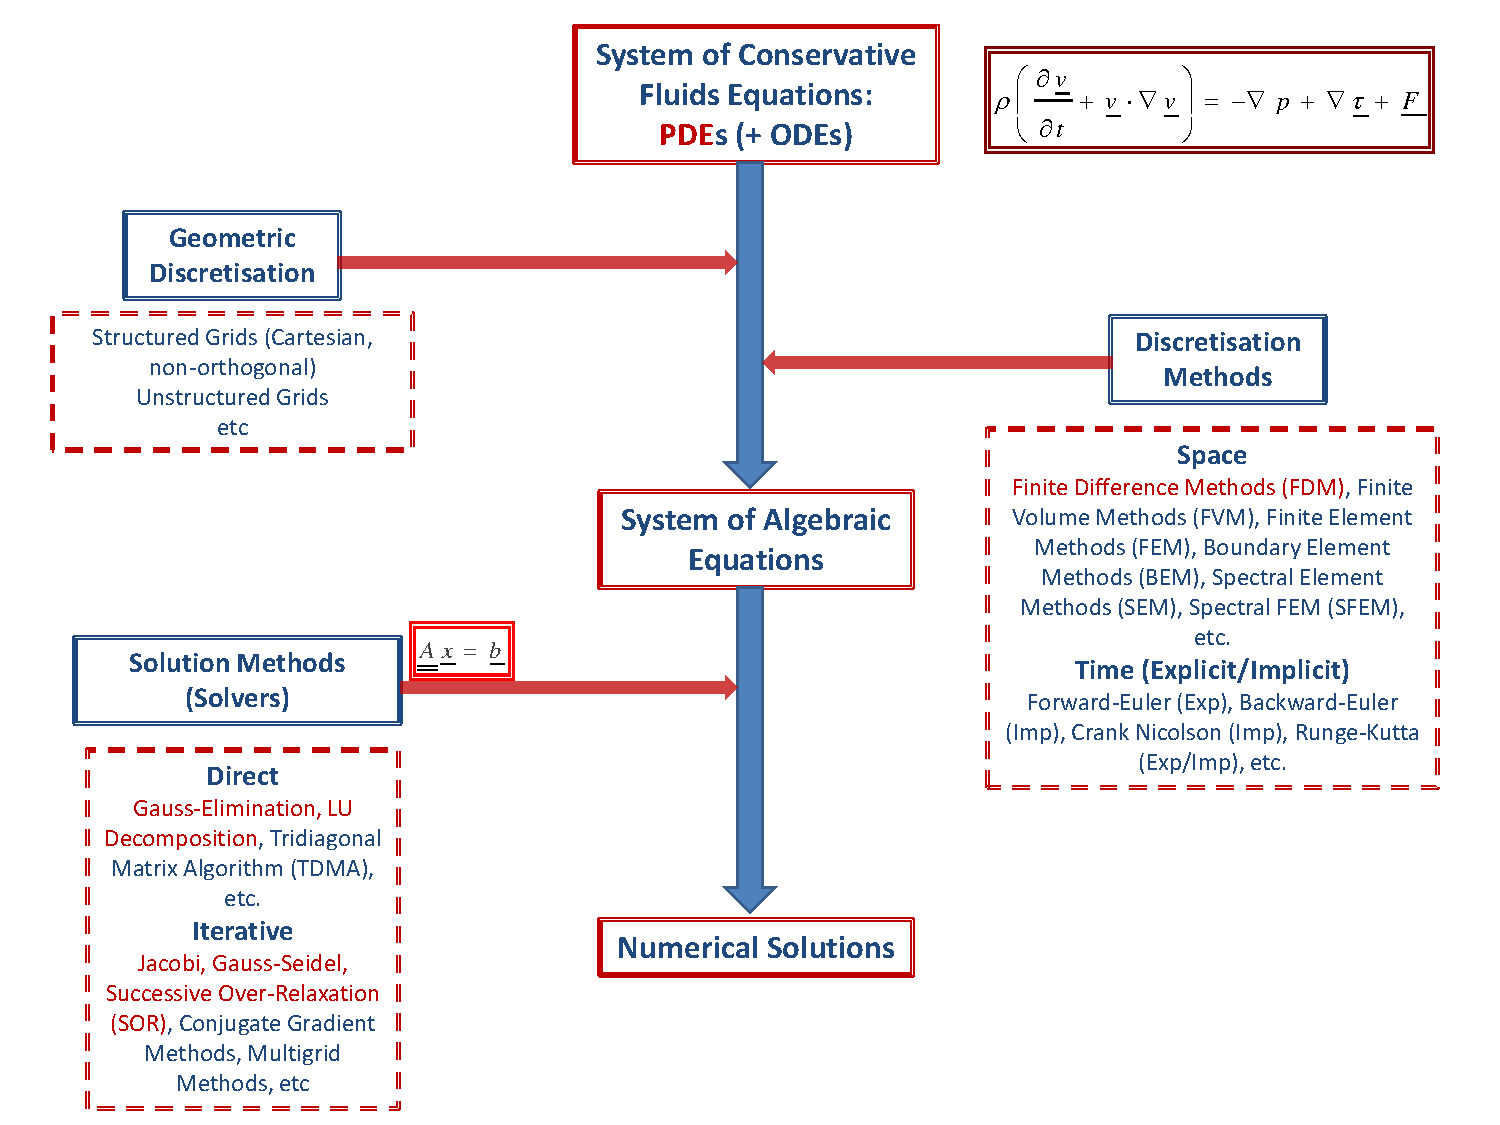
\includegraphics[width=12.cm, height=7.8cm, clip]{./Figs/CFD_Schematics2.pdf}
    \end{center}
%\caption{XX}
   \end{figure}    

\end{frame}


%##################
%%%   SUBSECTION
%##################
\subsection{Demonstration Problem}

%%%
%%% Slide
%%%
\begin{frame}
 \frametitle{Demonstration Problem: Laminar Pipe Flow} 

   \begin{figure}%
    \begin{center}
     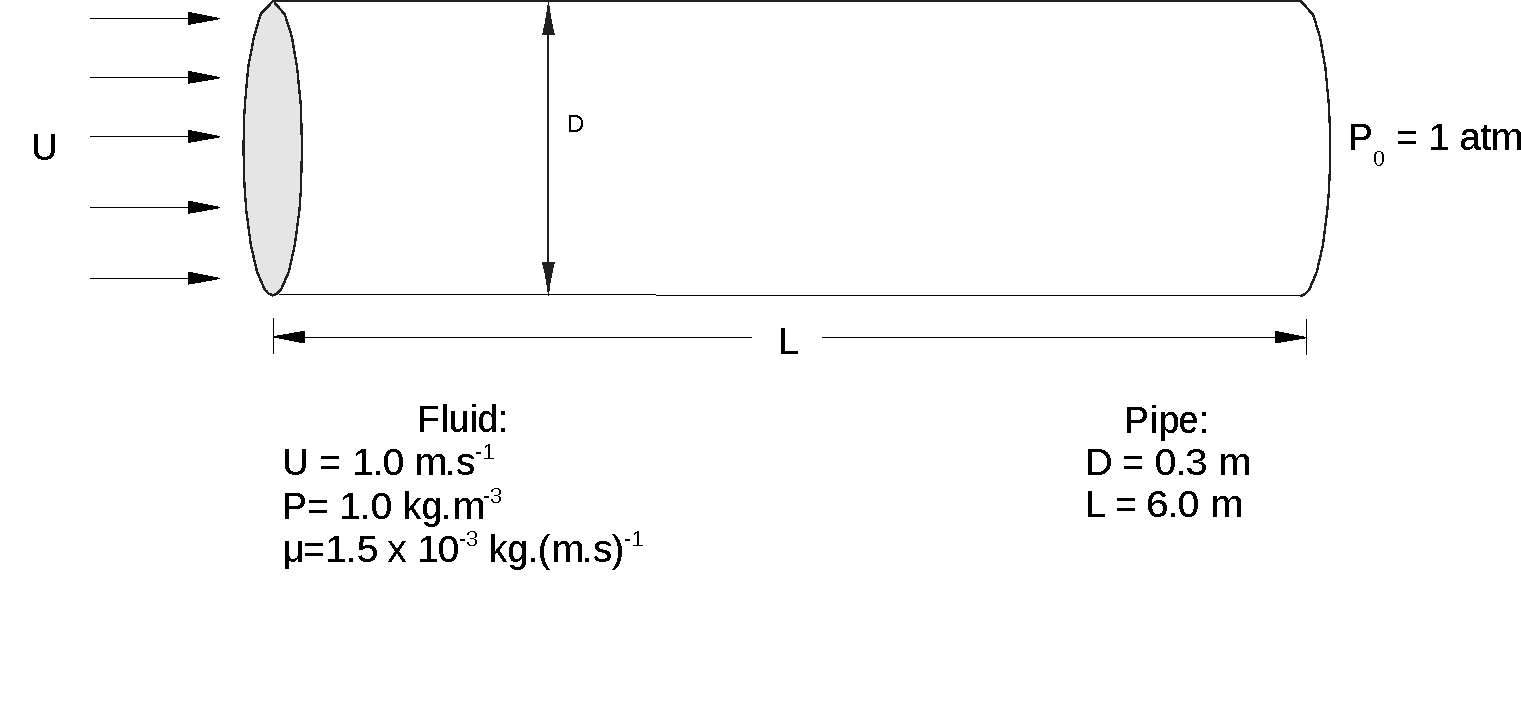
\includegraphics[width=8.cm, clip]{./Figs/LaminarPipeFlow2.pdf}
    \end{center}
   \end{figure}    
   \visible<2->{Note that these properties result in $Re=\frc{\rho D L}{\mu} = 200 \Rightarrow$\;\; \red{Laminar flow}. }

   \visible<3->{Solve this flow problem using \blue{ANSYS Fluent} to obtain the following information:}
       \begin{enumerate}[a)]
          \item<4-> velocity vectors;
          \item<4-> velocity magnitude contours;
          \item<4-> velocity profiles;
          \item<4-> skin friction coefficient along the pipe wall.
       \end{enumerate}
   \visible<4->{\blue{Compare these results with the analytic solution for fully developed laminar pipe flow}.}

\end{frame} 

%%%
%%% Slide
%%%
\begin{frame}
 \frametitle{Demonstration Problem: Laminar Pipe Flow} 
    \begin{columns}
       \begin{column}[l]{0.5\linewidth}
          \begin{description}\scriptsize
             \item[Windows Desktop:]<1-> Physical Sciences $\Longrightarrow$ Engineering $\Longrightarrow$ \blue{ANSYS 14.5} $\Longrightarrow$ Workbench 14.5;
             \item[ANSYS WorkBench:]<2-> {\it Toolbox Area} (left hand-side) and {\it Project Schematic} (main area);
             \item[Analysis System:]<3-> Contains the type of physical problems to be solved. We will select {\it Fluid Flow (Fluent)}.
             \item[Project Schematic Area:]<4-> The main area will contain all elements for the simulation:
                \begin{enumerate}[a)]\scriptsize
                   \item<5-> Geometry;
                   \item<5-> Mesh;
                   \item<5-> Setup;
                   \item<5-> Simulations and;
                   \item<5-> Results.
                \end{enumerate}
          \end{description}
       \end{column}
       \begin{column}[l]{0.5\linewidth}
          \visible<2->{\begin{figure}
                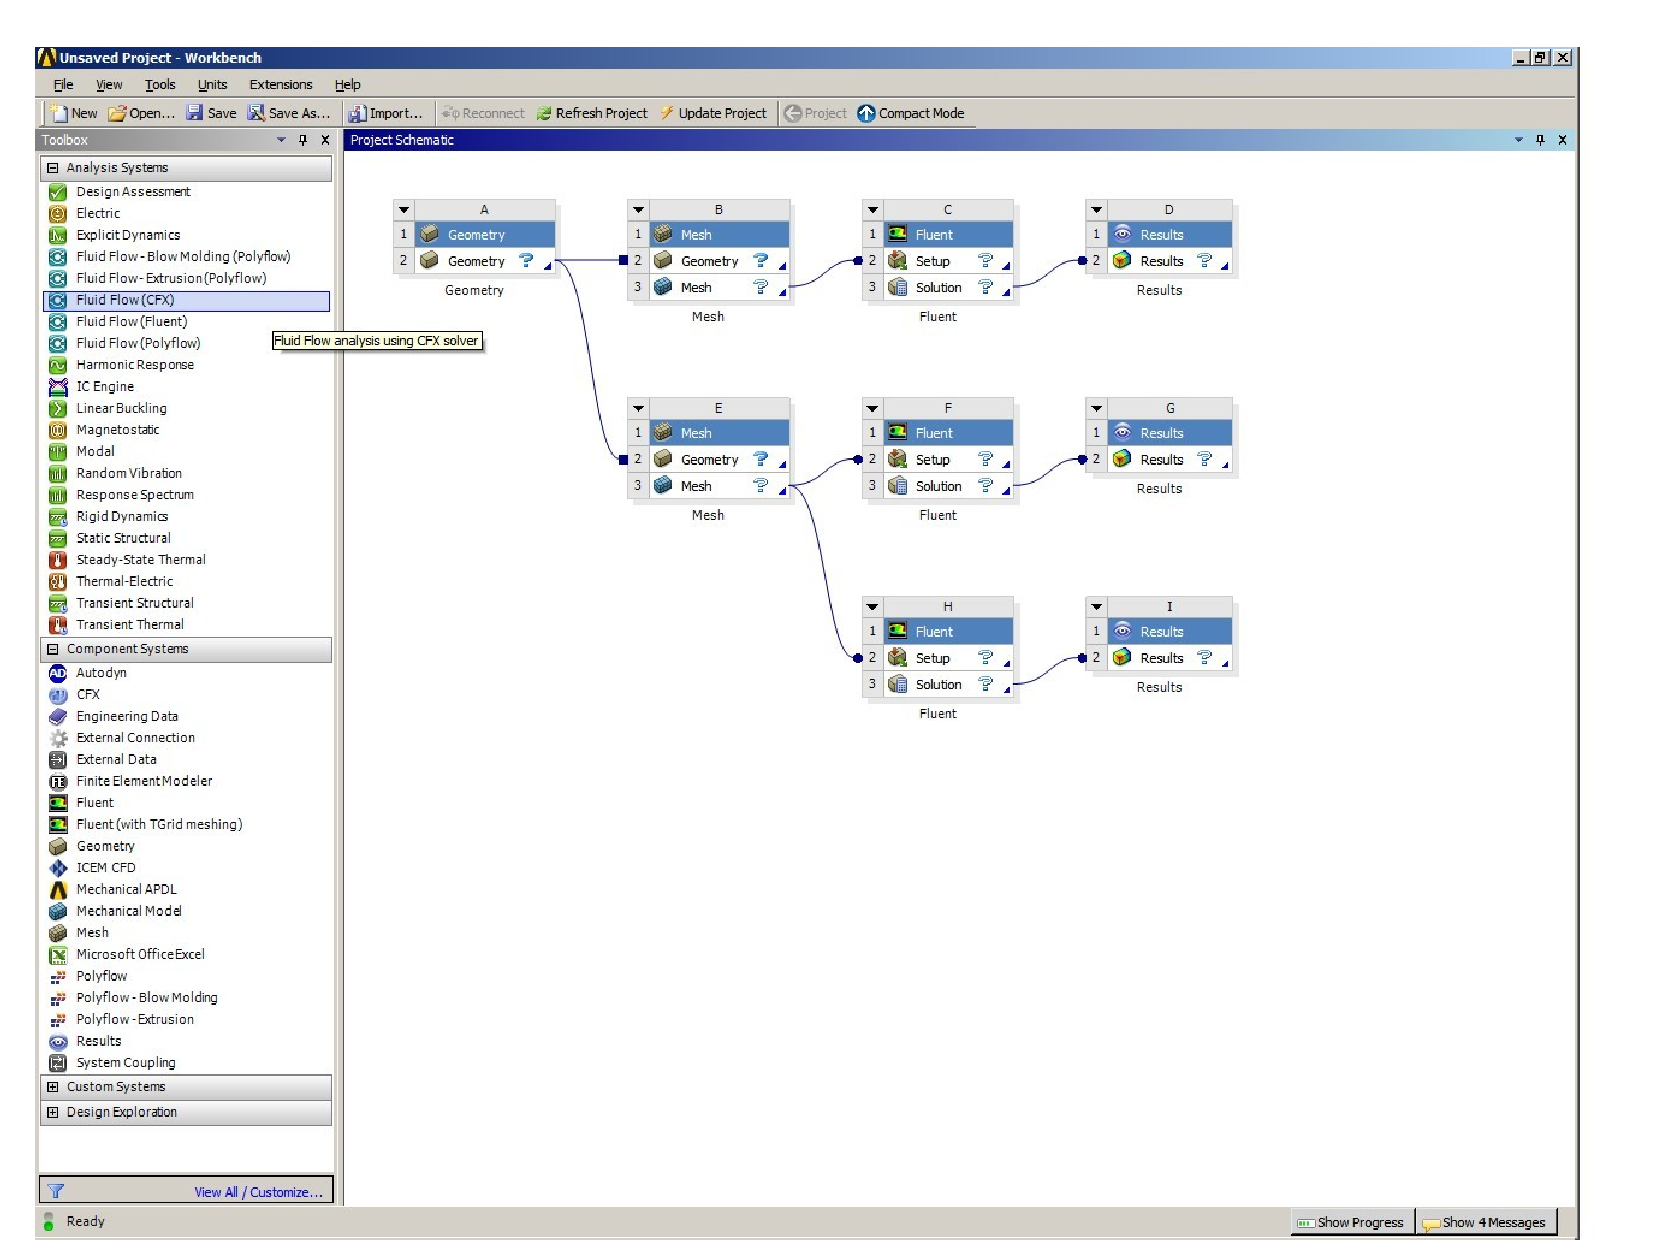
\includegraphics[width=\columnwidth, clip]{./Figs/SystemInitialisation_b.pdf} 
                \caption{Laminar pipe flow -- schematics.}\label{SchematicsPipe}
          \end{figure}}
       \end{column}
    \end{columns}
\end{frame} 
 

%##################
%%%   SUBSECTION
%##################
\subsection{Pre-Processing}

%%%
%%% Slide
%%%
\begin{frame}
 \frametitle{Pre-processing} 
\begin{enumerate}
  \item <1-> We start with a mathematical model that represents a physical system, via:
    \begin{enumerate}
      \item <2-> Mass, momentum and energy conservative equations (e.g., Navier-Stokes, Stokes, Darcy, Richards equations, etc);
      \item <3-> Parametrisation of system properties (e.g., equations of state to define fluid densities, algebraic expressions for viscosities, thermal conductivity, etc);
      \item <4-> General simplifying assumptions (e.g., inviscid / viscous, steady-state / transient, laminar / turbulent, 1-/2-/3-D, compressible/incompressible, etc); 
      \item <5-> Appropriate set of boundary and initial conditions.
    \end{enumerate}
  \item <6-> Discretise the geometry (mathematical domain) with mesh/grids containing cells (or elements or control volumes): 
    \begin{enumerate}
      \item <7-> 2-D: Triangle and quadrilateral;
      \item <8-> 3-D: Tetrahedron, hexahedron, pyramid, prism with triangular base, etc 
    \end{enumerate}
\end{enumerate} 
\begin{itemize}
   \item <9-> The mesh/grid can either be structured (i.e., regular connectivity), unstructured (i.e., irregular connectivity) and hybrid;
   \item <10-> The stage of: (a) designing the geometry that represents the physical problem, (b) meshing the designed geometry; (c) input initial and boundary conditions; (d) prescribed operation conditions and (e) solver options \textcolor{red}{$\Longrightarrow$} is also called \textcolor{blue}{\underline{Pre-processing}}.
\end{itemize}  
\end{frame}

%######################
%%%   SUBSUBSECTION
%######################
\subsubsection{Pre-Processing: Geometry Setup}
 
%%%
%%% Slide
%%%
\begin{frame}
 \frametitle{Pre-processing: Geometry Setup} 
    \begin{columns}
       \begin{column}[l]{0.5\linewidth}
          \begin{enumerate}[1)]\scriptsize
             \item<1-> Establish the dimension of the problem:
                 \begin{enumerate}[a)]\scriptsize
                    \item<1-> Drag \blue{Geometry} from the \blue{Component Systems} menu to the main area;
                    \item<1-> Right-click \blue{Geometry} $\rightarrow$ \blue{Properties}
                    \item<1-> Select \red{2D};
                 \end{enumerate}
             \item<2-> Establish the unit for the geometry:
                 \begin{enumerate}[a)]\scriptsize
                    \item<2-> Right-click \blue{Geometry} $\rightarrow$ \blue{New Geometry}
                    \item<2-> Select \red{Meter};
                 \end{enumerate}
          \end{enumerate}
       \end{column}
       \begin{column}[l]{0.5\linewidth}
          \visible<1->{\begin{figure}
                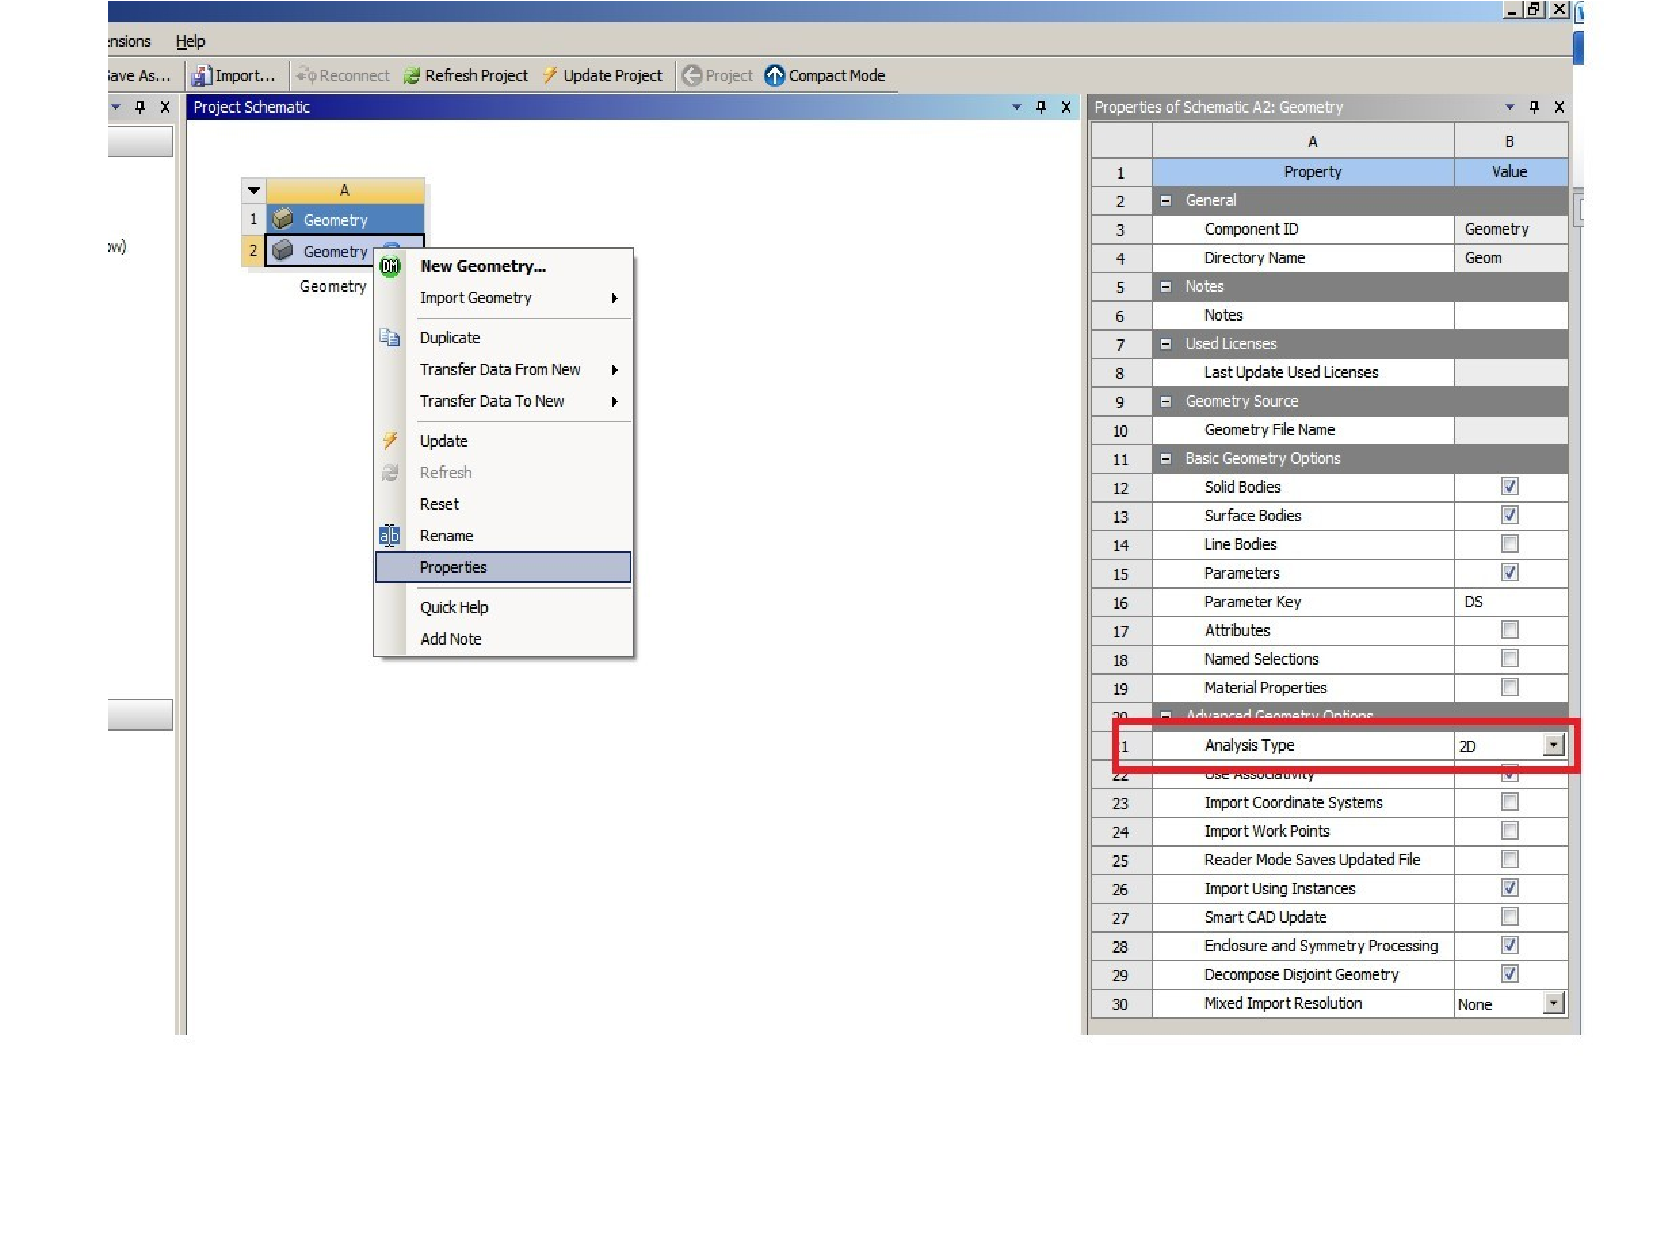
\includegraphics[width=\columnwidth, clip]{./Figs/Geometry.pdf} 
          \end{figure}}
       \end{column}
    \end{columns}
\end{frame} 
 
%%%
%%% Slide
%%%
\begin{frame}
 \frametitle{Pre-processing: Geometry Setup} 
    \begin{columns}
       \begin{column}[l]{0.5\linewidth}
          \begin{enumerate}[1)]\scriptsize\setcounter{enumi}{2}
             \item<1-> In the \blue{DesignModeler}, we can start creating the required geometry:
                 \begin{enumerate}[a)]\scriptsize
                    \item<1-> Select \blue{XYplane} from the \blue{Tree Outline} field;
                    \item<1-> Click in the \blue{New Sketch} symbol from the \blue{Sketch Toolbar} $\Rightarrow$ \blue{Sketch1};
                 \end{enumerate}
             \item<2-> In order to adjust the visualisation of the sketch geometry, we should select \blue{Z-axis} to obtain a \blue{XYPlane} visualisation;
          \end{enumerate}
          \begin{center}
                \visible<1->{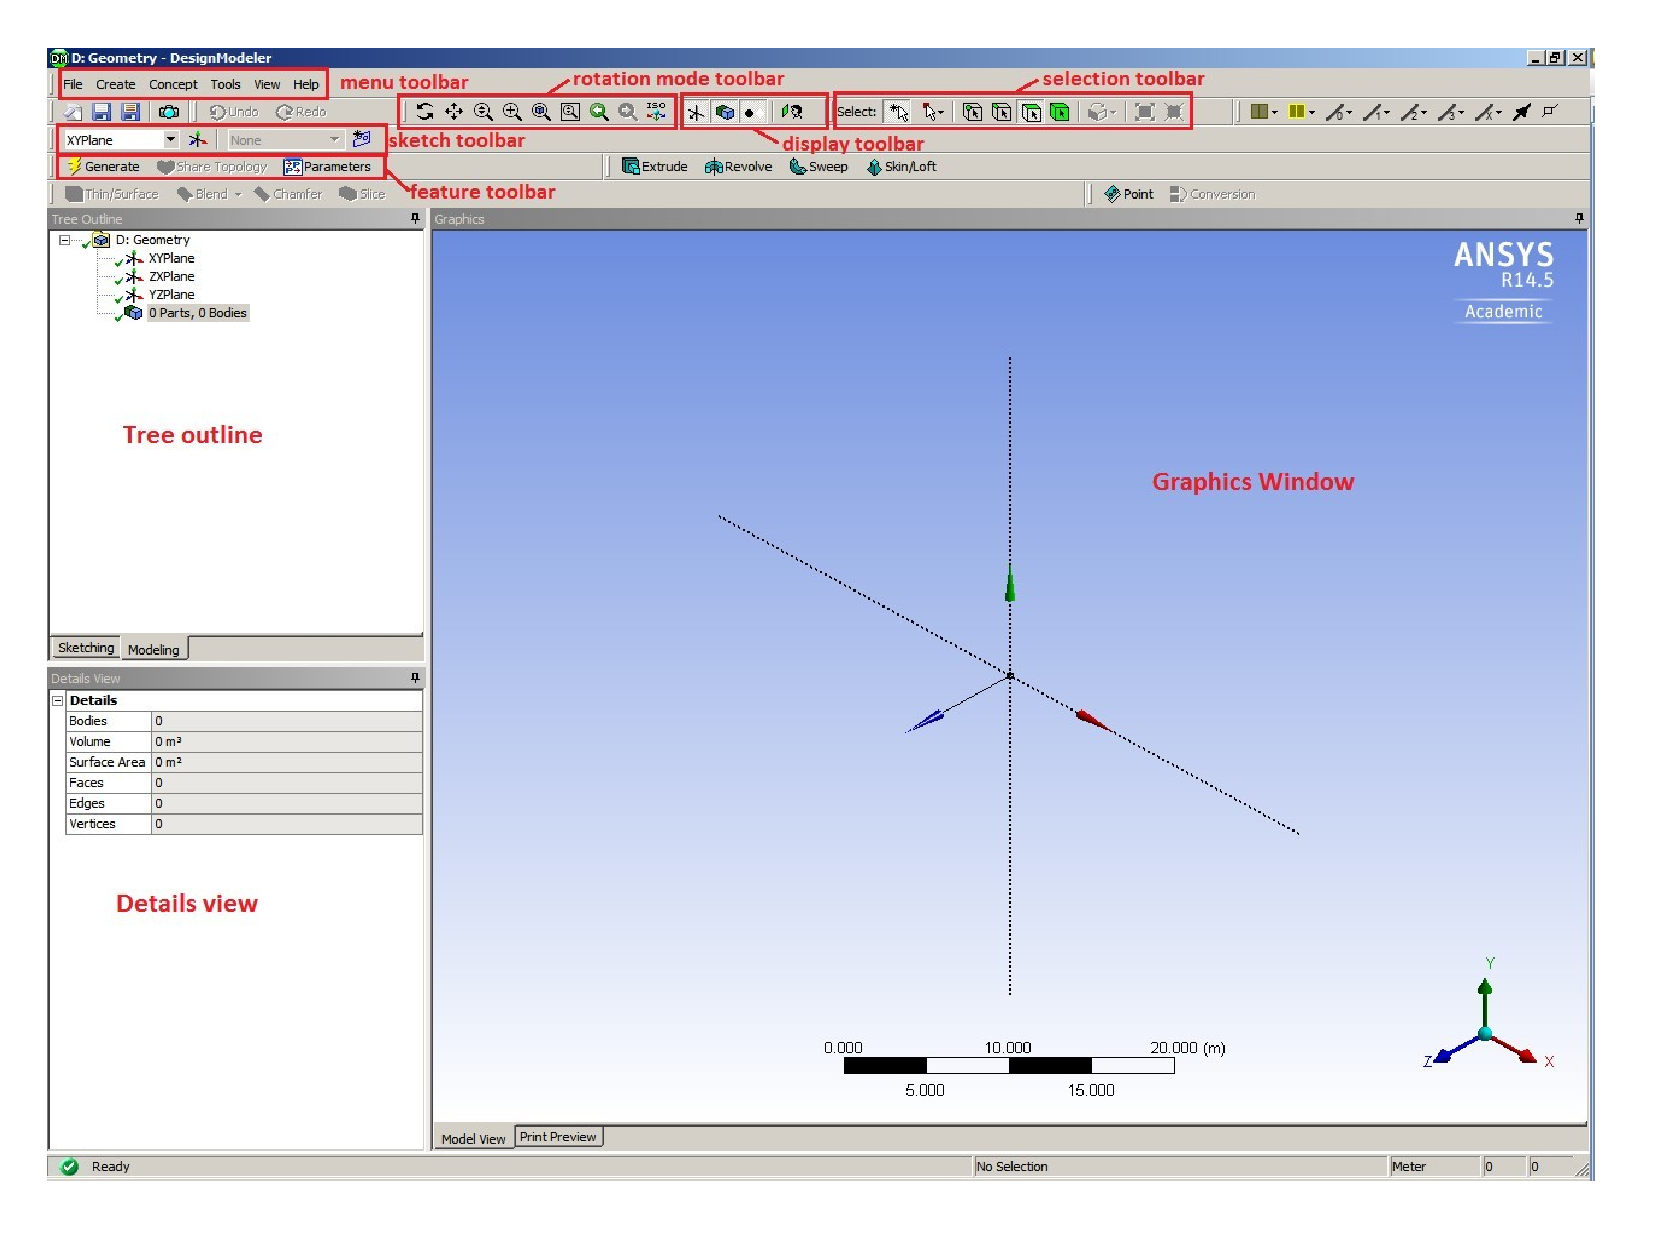
\includegraphics[width=.8\columnwidth, clip]{./Figs/Geometry2.pdf}}
          \end{center}
       \end{column}
       \begin{column}[l]{0.5\linewidth}
          \begin{enumerate}[1)]\scriptsize\setcounter{enumi}{4} 
             \item<3-> Generating the Geometry:
                 \begin{enumerate}[a)]\scriptsize
                    \item<3-> Select \blue{Rectangle} and draw the rectangle that will represent the pipe (Fig.~\ref{SchematicsPipe}). 
                    \item<3-> \blue{P} indicates the origin of the geometry;
                    \item<3-> As the mouse `touch' the lines, a letter \blue{C} will also appear;
                 \end{enumerate}
          \end{enumerate} 
          \begin{center}
                \visible<3->{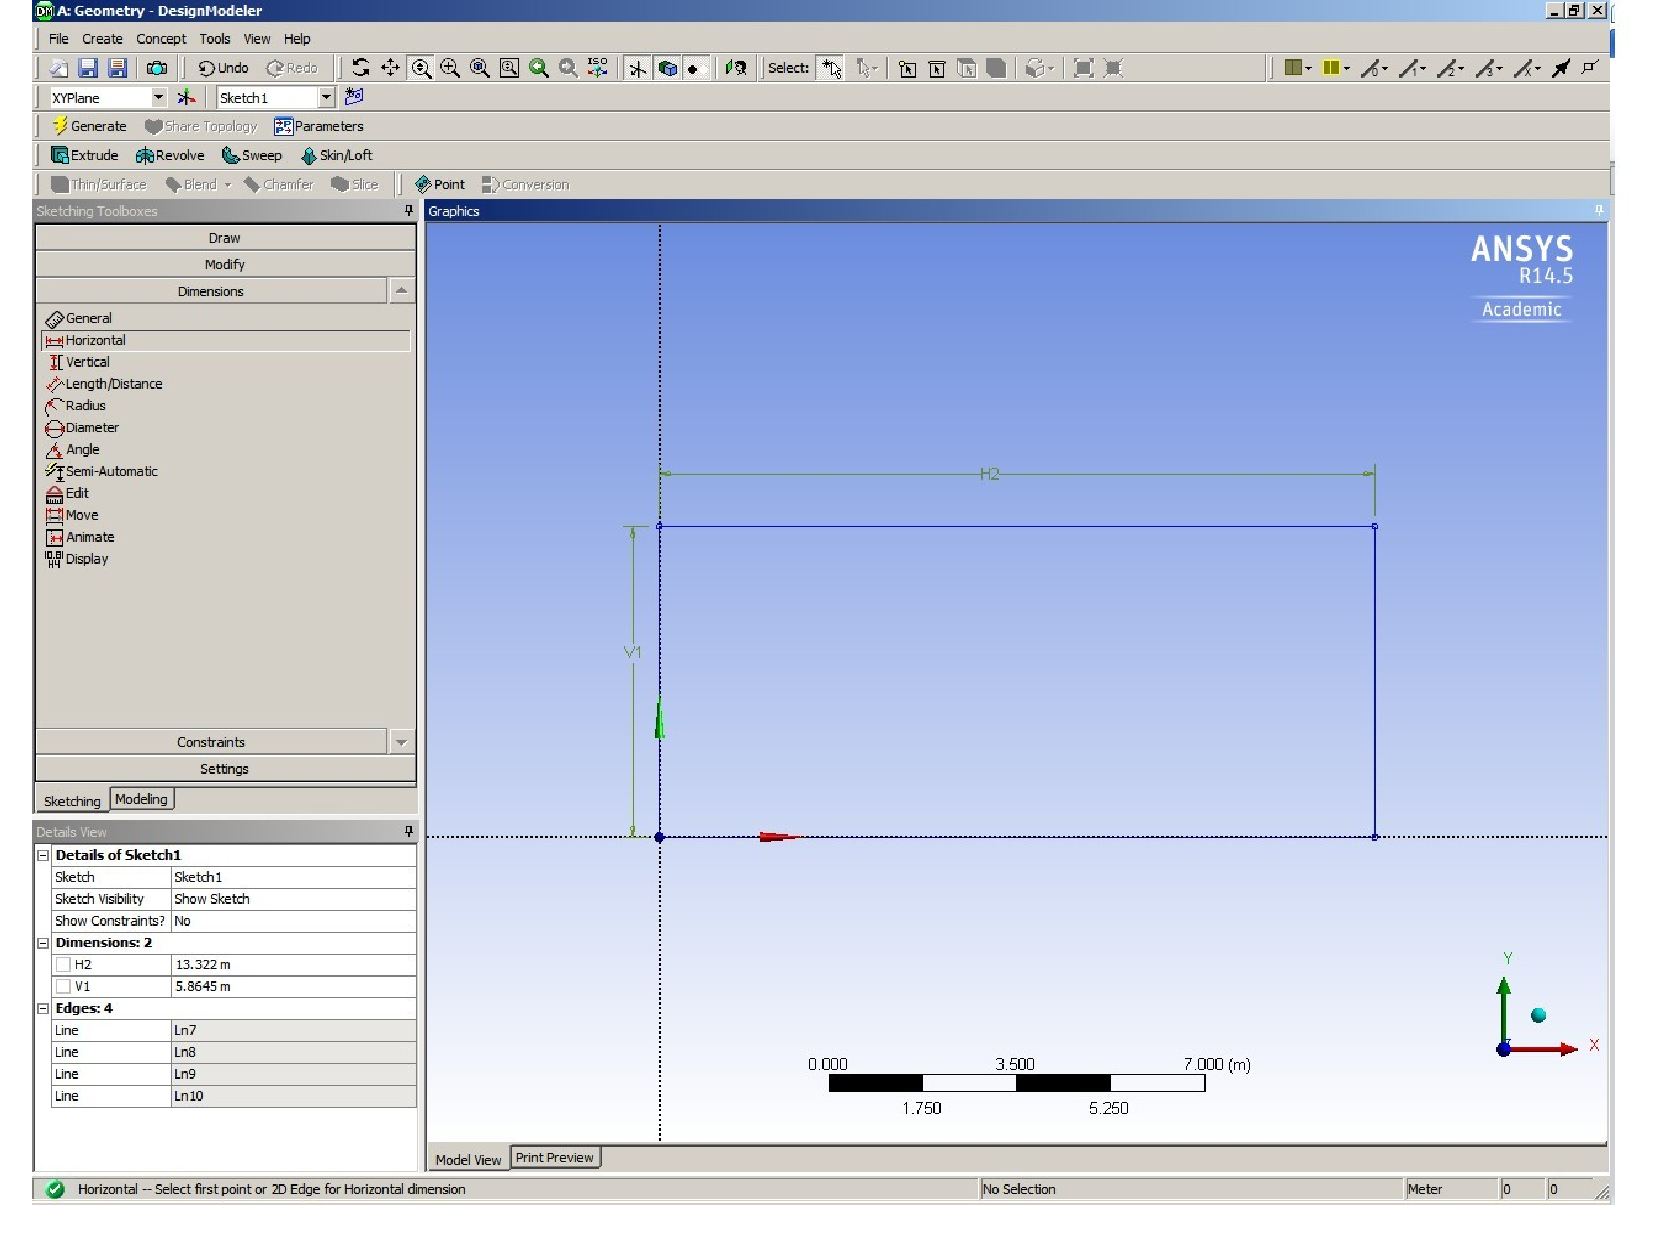
\includegraphics[width=.8\columnwidth, clip]{./Figs/Geometry3.pdf}}
          \end{center}
       \end{column}
    \end{columns}

\end{frame} 


 
%%%
%%% Slide
%%%
\begin{frame}
 \frametitle{Pre-processing: Geometry Setup} 
    \begin{columns}
       \begin{column}[l]{0.5\linewidth}
          \begin{enumerate}\scriptsize\setcounter{enumi}{5}
             \item<1-> Setting dimensions of the rectangle:
                 \begin{enumerate}[a)]\scriptsize
                    \item<1-> Select \blue{Dimensions menu} from the \blue{Sketching Tab};
                    \item<1-> Select \blue{Vertical} and click in the upper and lower line boundaries of the rectangle. Click on \blue{V1} symbol;
                    \item<1-> Repeat the procedure for the horizontal dimension by selecting \blue{Horizontal} in the \blue{Sketching Tab};
                    \item<1-> In the \blue{Details View table}, set $H2 = 6$ m and $V1 = 0.15$ m $= r = \frc{D}{2}$.
                 \end{enumerate}
          \end{enumerate}
          \visible<1->{\begin{center}
                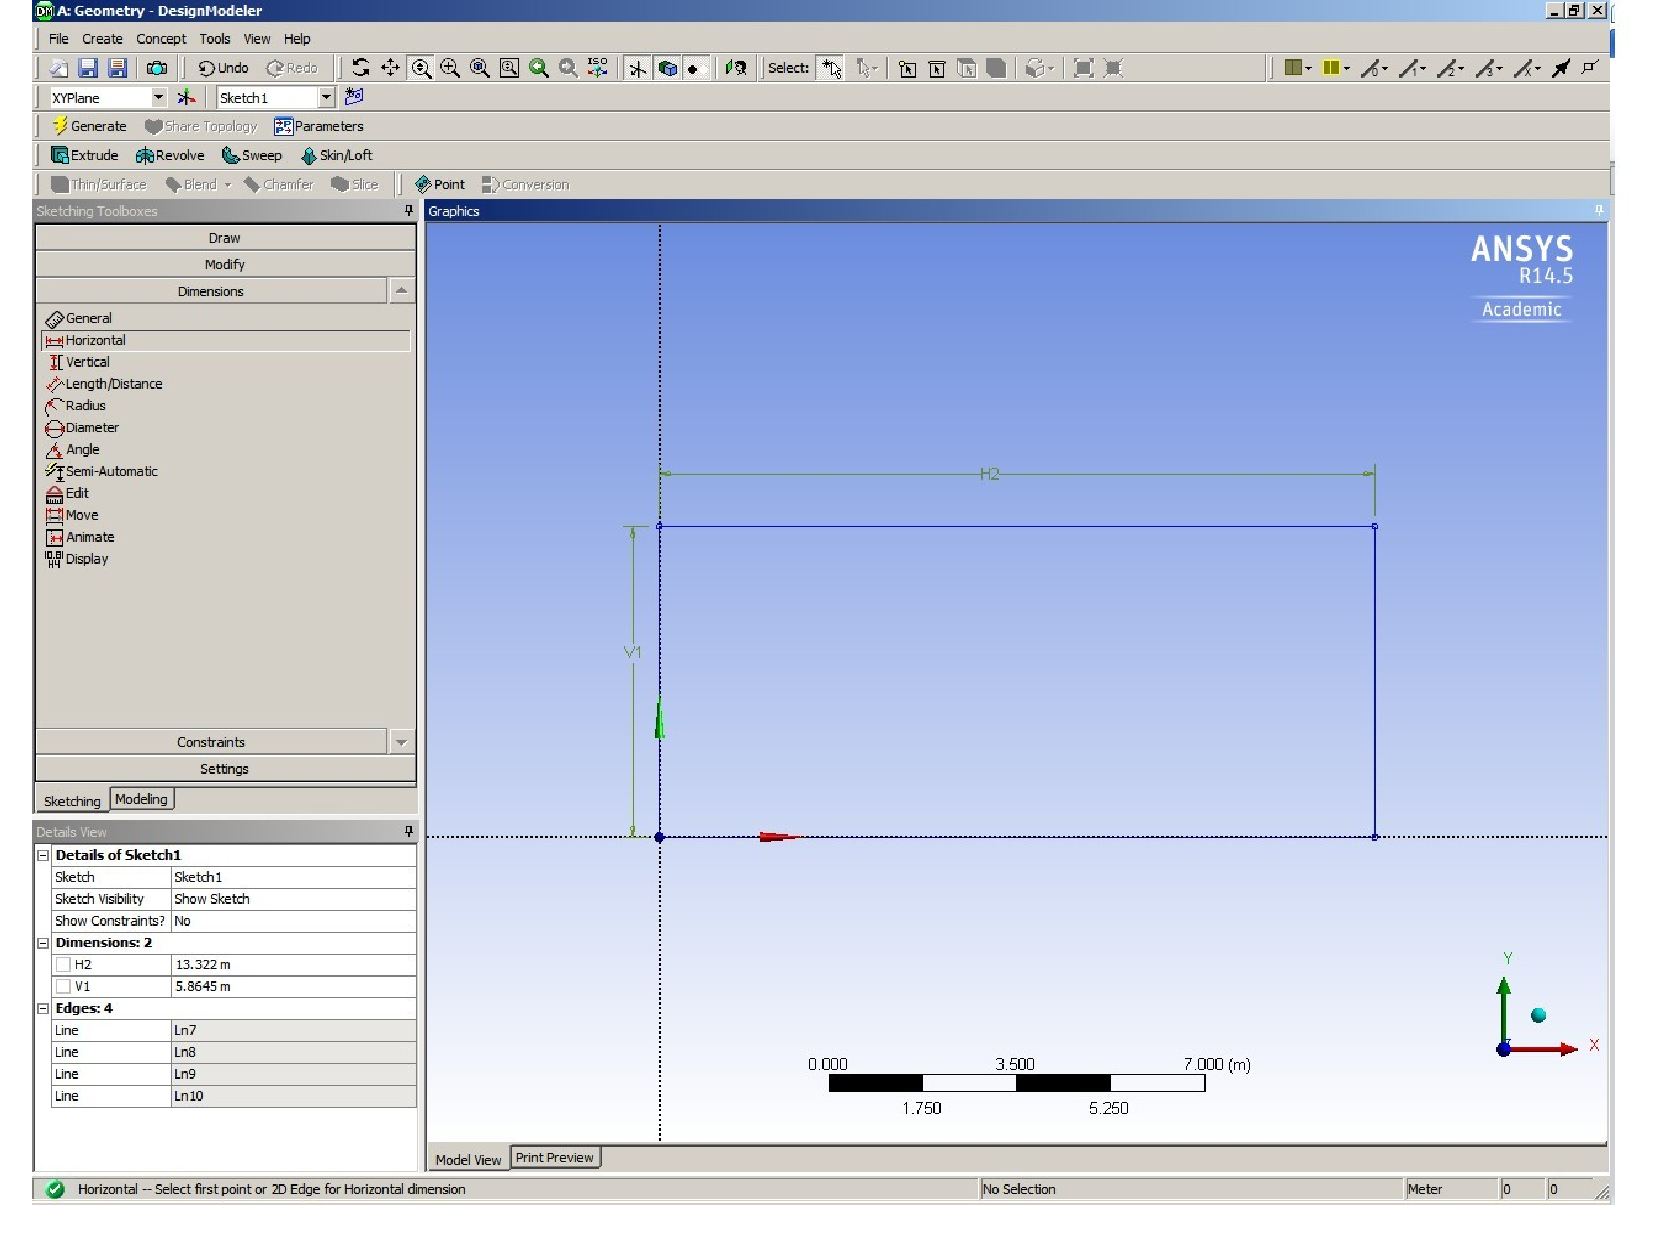
\includegraphics[width=.9\columnwidth, clip]{./Figs/Geometry3.pdf} 
          \end{center}}
       \end{column}
       \begin{column}[l]{0.5\linewidth}
          \visible<2->{\begin{center}
                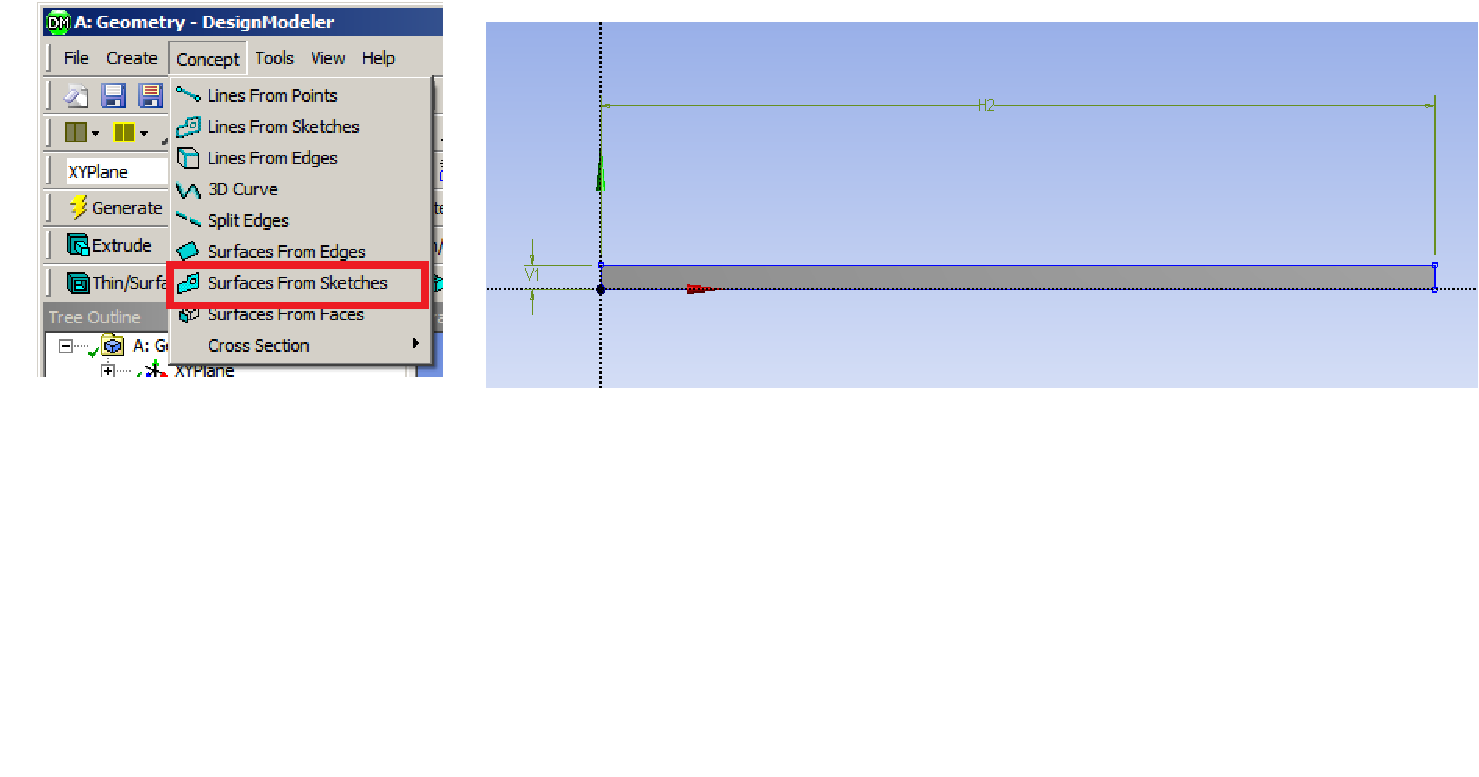
\includegraphics[width=\columnwidth, clip]{./Figs/Geometry4b.pdf} 
          \end{center}}
          \begin{enumerate}\scriptsize\setcounter{enumi}{6}
             \item<2-> Creating a \red{surface}:
                 \begin{enumerate}[a)]\scriptsize
                    \item<2-> Select \blue{Sketch1} from the \blue{Tree Outline};
                    \item<2-> All sides of the created rectangle should turn \blue{yellow};
                    \item<2-> Select \blue{Concept} $\Rightarrow$ \blue{Surfaces from Sketches};
                    \item<2-> Select \blue{Apply} and click on \blue{Generate icon} from the \blue{Feature Toolbar}.
                 \end{enumerate}
             \item<3-> Close the \blue{DesignModeler} and \red{save} the project;
             \item<3-> The project (for now, just the geometry) is contained in the file with extension $\ast$.wbpj.
          \end{enumerate}
       \end{column}
    \end{columns}
\end{frame} 

 
%######################
%%%   SUBSUBSECTION
%######################
\subsubsection{Pre-Processing: Mesh Generation}

%%%
%%% Slide
%%%
\begin{frame}
 \frametitle{Pre-processing: Mesh Generation}

   \begin{figure}%
    \begin{center}
     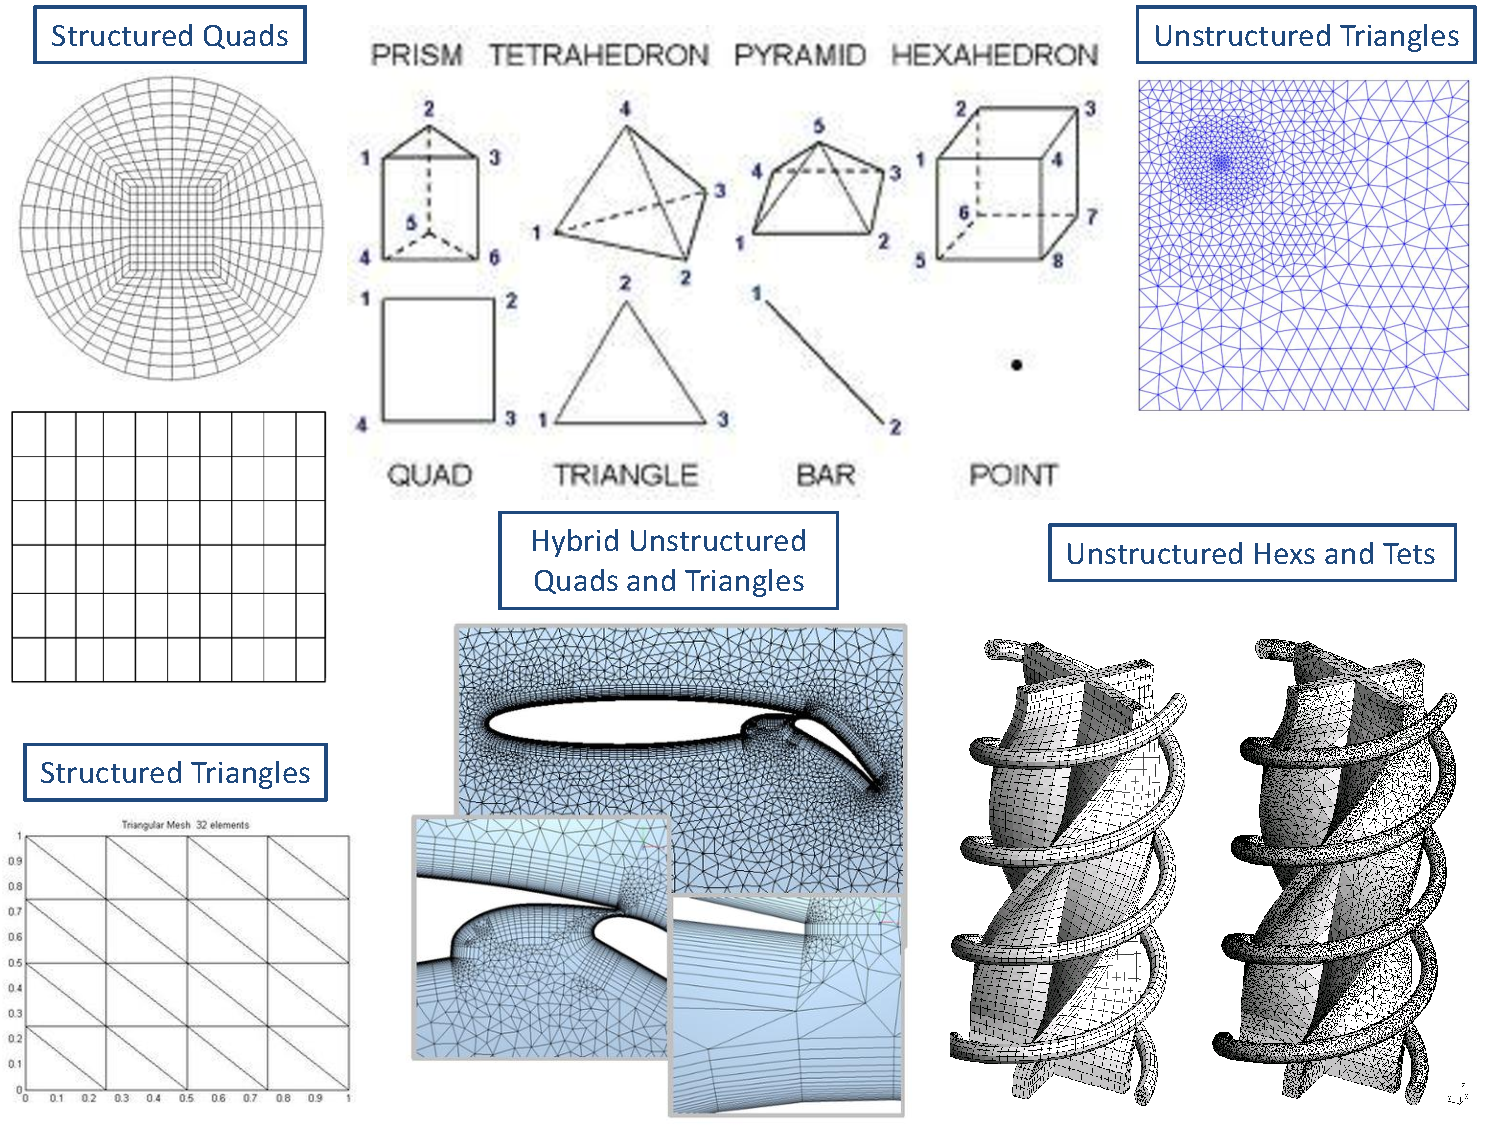
\includegraphics[width=12.cm, height=7.8cm, clip]{./Figs/MeshGrid_Examples.pdf}\label{xx}
    \end{center}
%\caption{XX}
   \end{figure}    

\end{frame}
%%%
%%% Slide
%%%
\begin{frame}
 \frametitle{Pre-processing: Mesh Generation} 
    \begin{columns}
       \begin{column}[l]{0.5\linewidth}
          \begin{enumerate}\scriptsize
             \item<1-> The conservative equations will be effectively solved in {\it each cell} of the mesh within the geometry;
             \item<1-> After generating the geometry, we now need to associate this geometry with a mesh:
                \begin{enumerate}[a)]\scriptsize
                   \item<2-> Drag the \blue{Mesh} component from the \blue{Component Systems menu} to the \blue{Project Schematic} area;
                   \item<2-> Establish a link between the existent \blue{Geometry box} and the \blue{new box}; 
                   \item<2-> Right-click \blue{Mesh cell} $\rightarrow$ \blue{Refresh}. This will link the geometry with mesh; 
                   \item<2-> Right-click \blue{Mesh} $\rightarrow$ \blue{Edit} $\Longrightarrow$ \blue{Meshing Window}.
                \end{enumerate}
          \end{enumerate}
       \end{column}
       \begin{column}[l]{0.5\linewidth}
          \visible<2->{\begin{figure}
                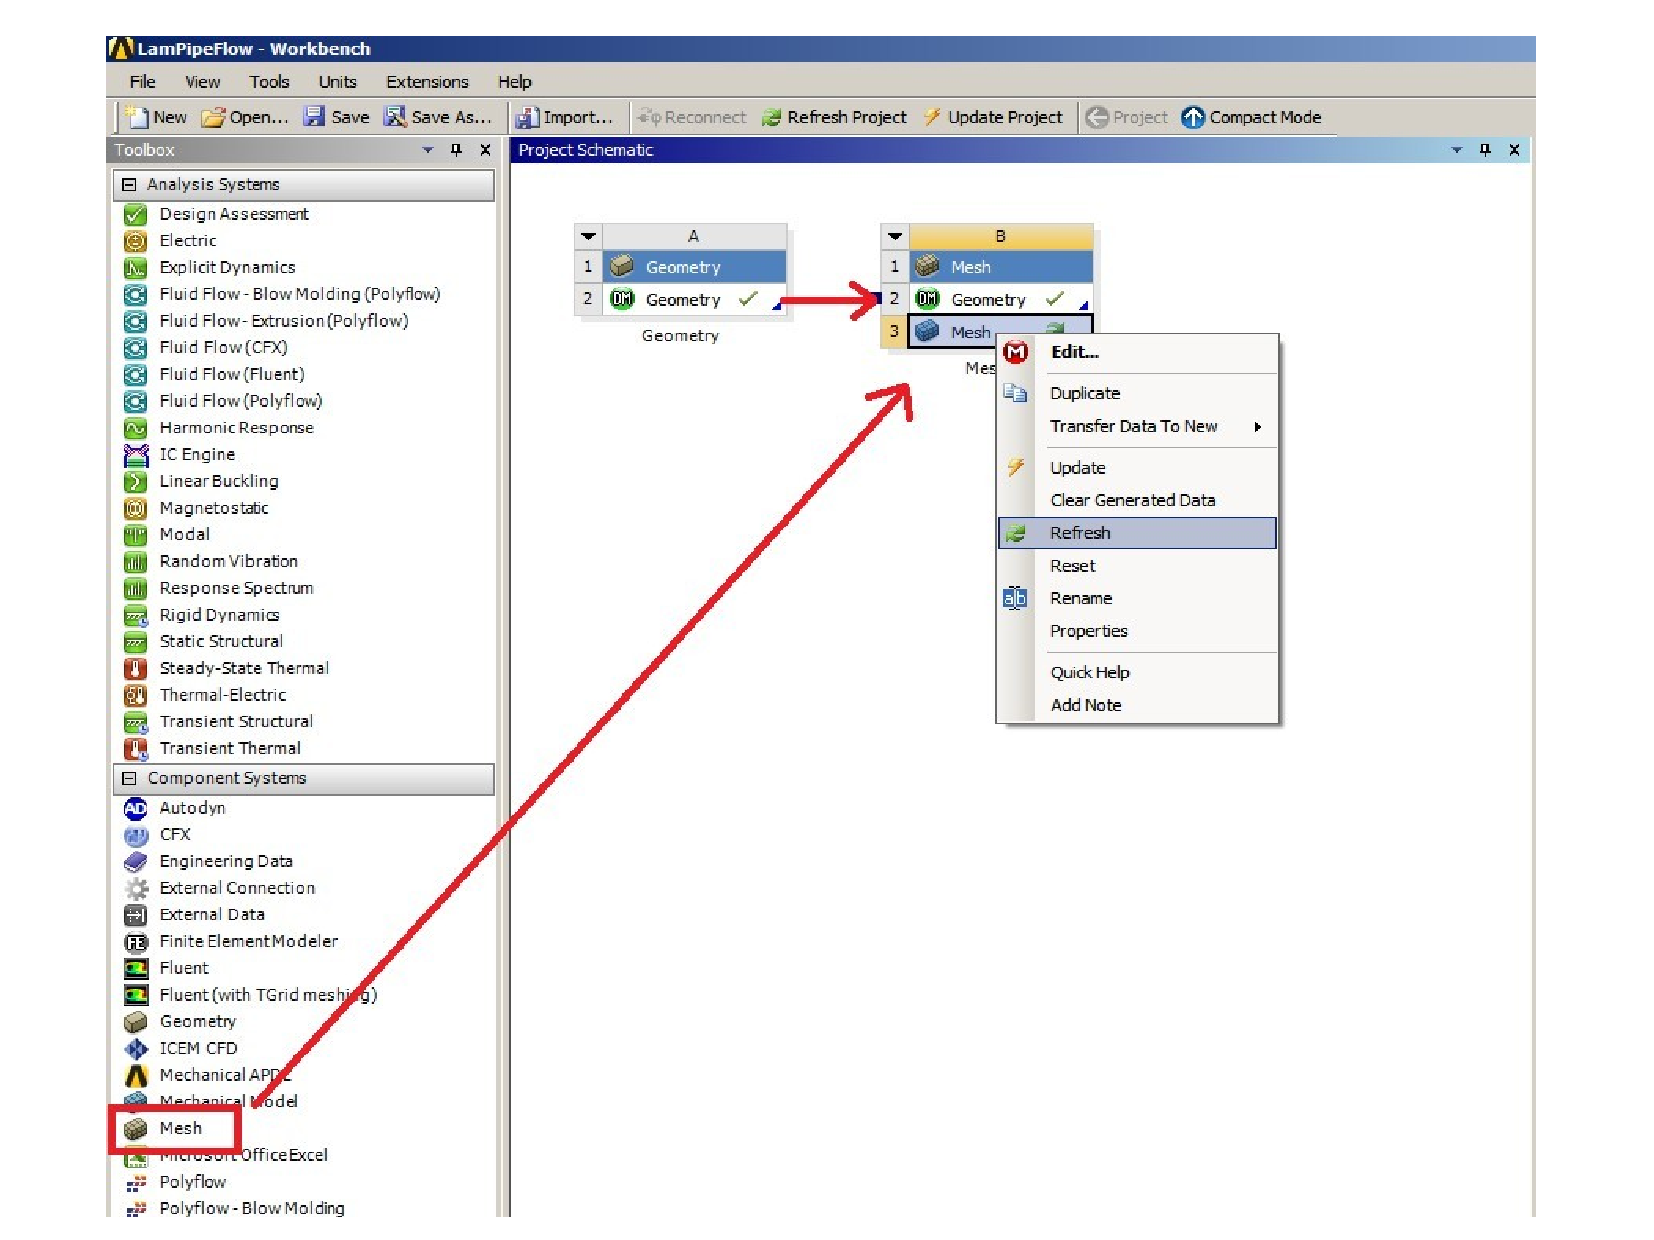
\includegraphics[width=1.1\columnwidth, clip]{./Figs/MeshGeneration1.pdf} 
          \end{figure}}
       \end{column}
    \end{columns}
\end{frame} 

 
%%%
%%% Slide
%%%
\begin{frame}
 \frametitle{Pre-processing: Mesh Generation} 
    \begin{columns}
       \begin{column}[l]{0.5\linewidth}
          \begin{enumerate}\scriptsize\setcounter{enumi}{2}
             \item<1-> Creating boundary lines:
                \begin{enumerate}[a)]\scriptsize
                   \item<2-> Click the \blue{Edge Tool symbol} from the \blue{Selection Toolbar};
                   \item<2-> Click in the {\it left edge of the geometry} in the \blue{Geometry window};
                   \item<2-> Right-click the \underline{green highlighted line} and select \blue{Create Named Selection};
                   \item<3-> Name the boundary \red{Inlet} in the \blue{Selection name window};
                   \item<3-> Repeat the procedure with the other three boundaries, naming \red{Pipewall} (upper boundary), \red{Outlet} (rhs) and \red{Centreline} (lower boundary).
                \end{enumerate}
          \end{enumerate}
       \end{column}
       \begin{column}[l]{0.5\linewidth}
          \vbox{\vspace{-0.5cm}
          \visible<2->{\begin{center}
                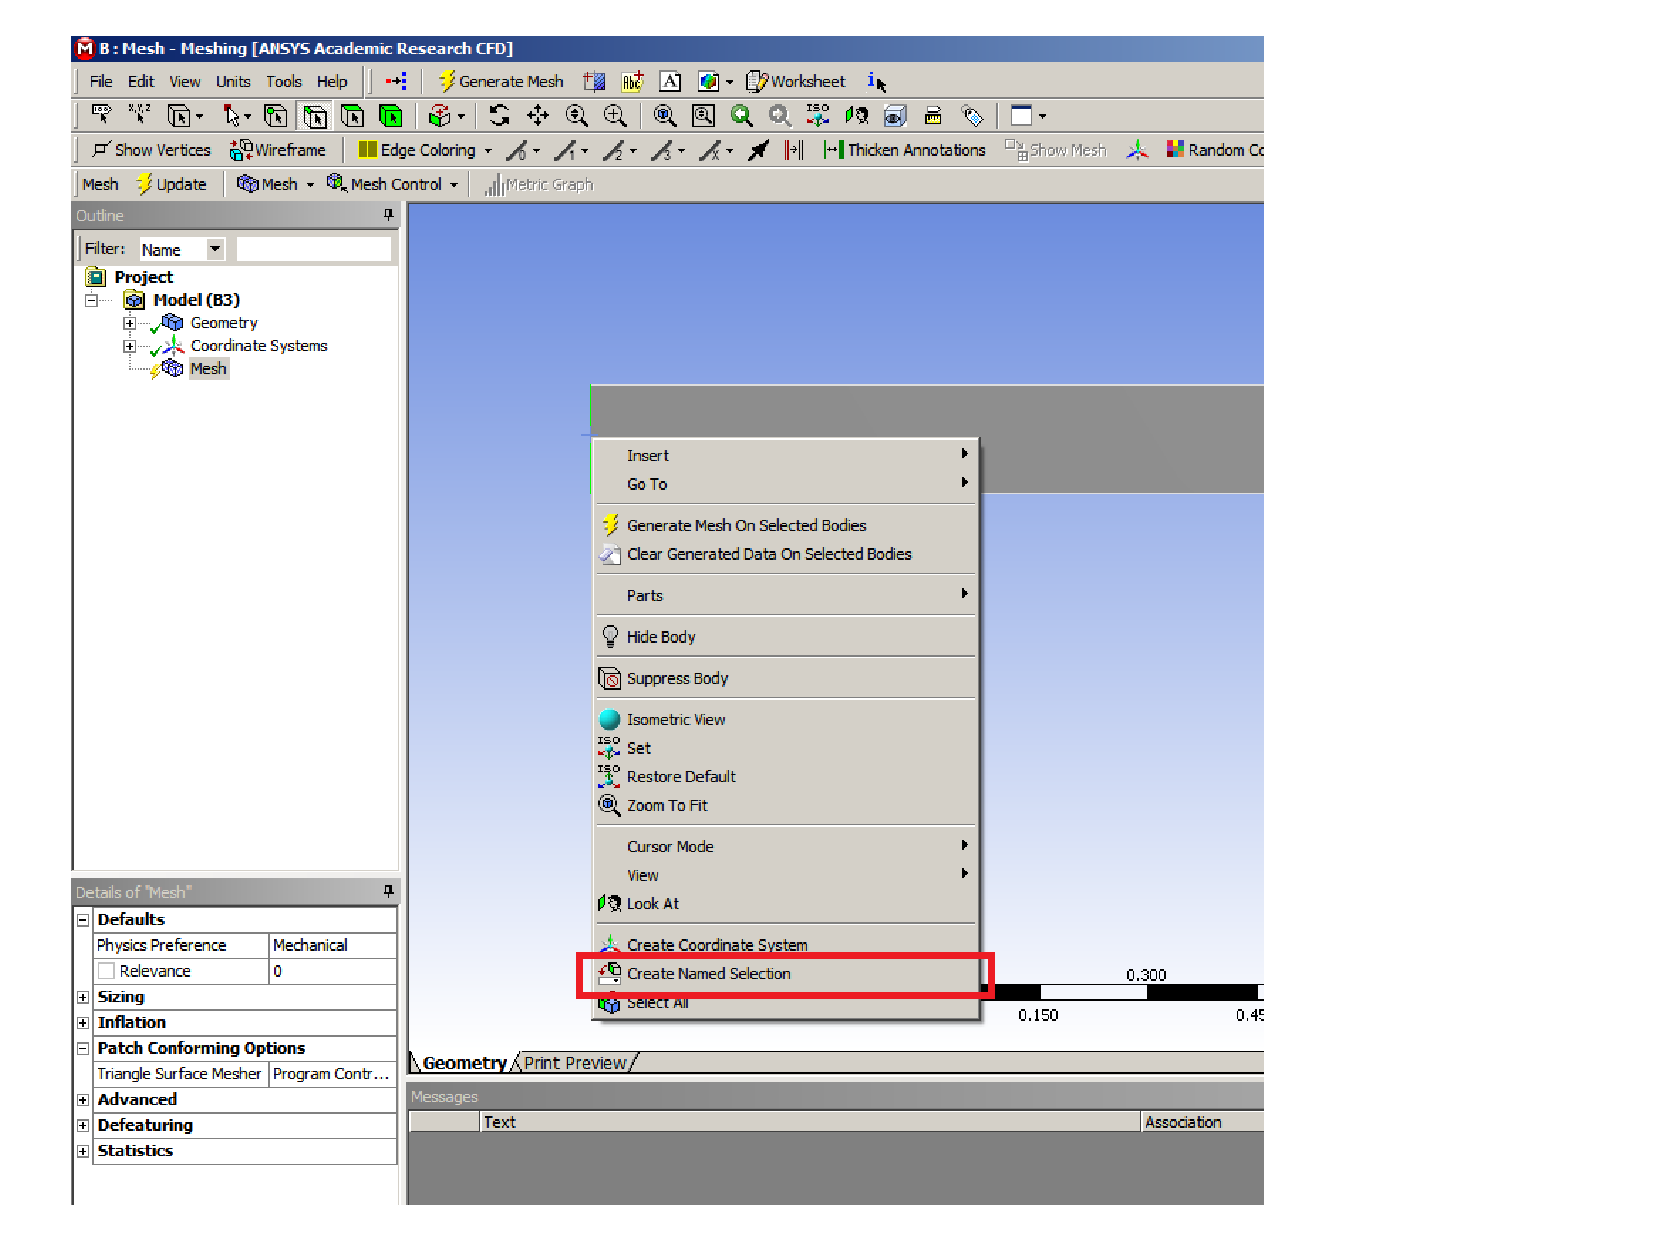
\includegraphics[width=\columnwidth, clip]{./Figs/MeshGeneration2.pdf} 
          \end{center}}\vspace{-0.7cm}
          \visible<3->{\begin{center}
                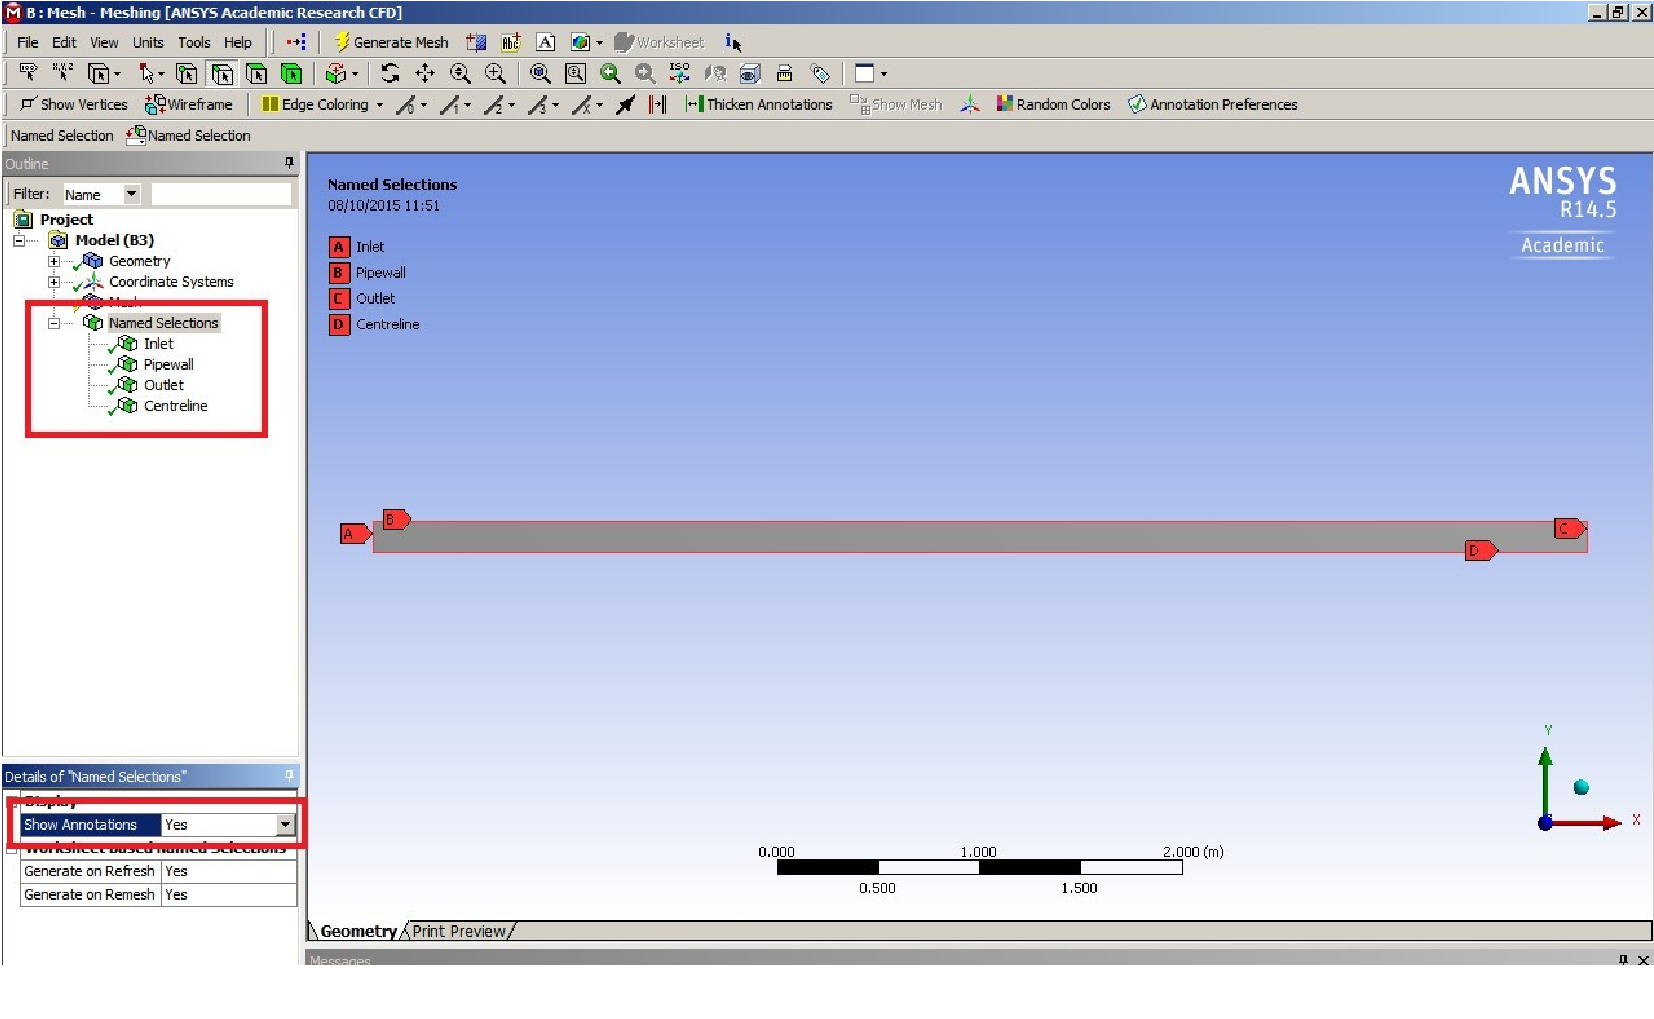
\includegraphics[width=\columnwidth, clip]{./Figs/MeshGeneration3.pdf} 
          \end{center}}}
       \end{column}
    \end{columns}
\end{frame} 

 
%%%
%%% Slide
%%%
\begin{frame}
 \frametitle{Pre-processing: Mesh Generation} 
    \begin{columns}
       \begin{column}[l]{0.5\linewidth}
          \begin{enumerate}\scriptsize\setcounter{enumi}{3}
             \item<1-> Creating uniform structured mesh:
                \begin{enumerate}[a)]\scriptsize
                   \item<2-> Right-click \blue{Mesh} from the \blue{Tree Outline};
                   \item<2-> Select \blue{Insert} $\Rightarrow$ \blue{Mapped Face Meshing};
                \end{enumerate}
             \item<3-> Applying the meshto the whole pipe geometry:
                \begin{enumerate}[a)]\scriptsize
                   \item<3-> Click on the pipe face in the \blue{Geometry Window}. The selected face will turn \red{green};
                   \item<3-> Click on \blue{No selection} in the \red{yellow} \blue{Geometry} cell from the \blue{Details View} menu $\rightarrow$ \blue{Apply};
                   \item<3-> \blue{Geometry cell} face should turn blue.
                \end{enumerate}
          \end{enumerate}
       \end{column}
       \begin{column}[l]{0.5\linewidth}
          \visible<2->{\begin{figure}
                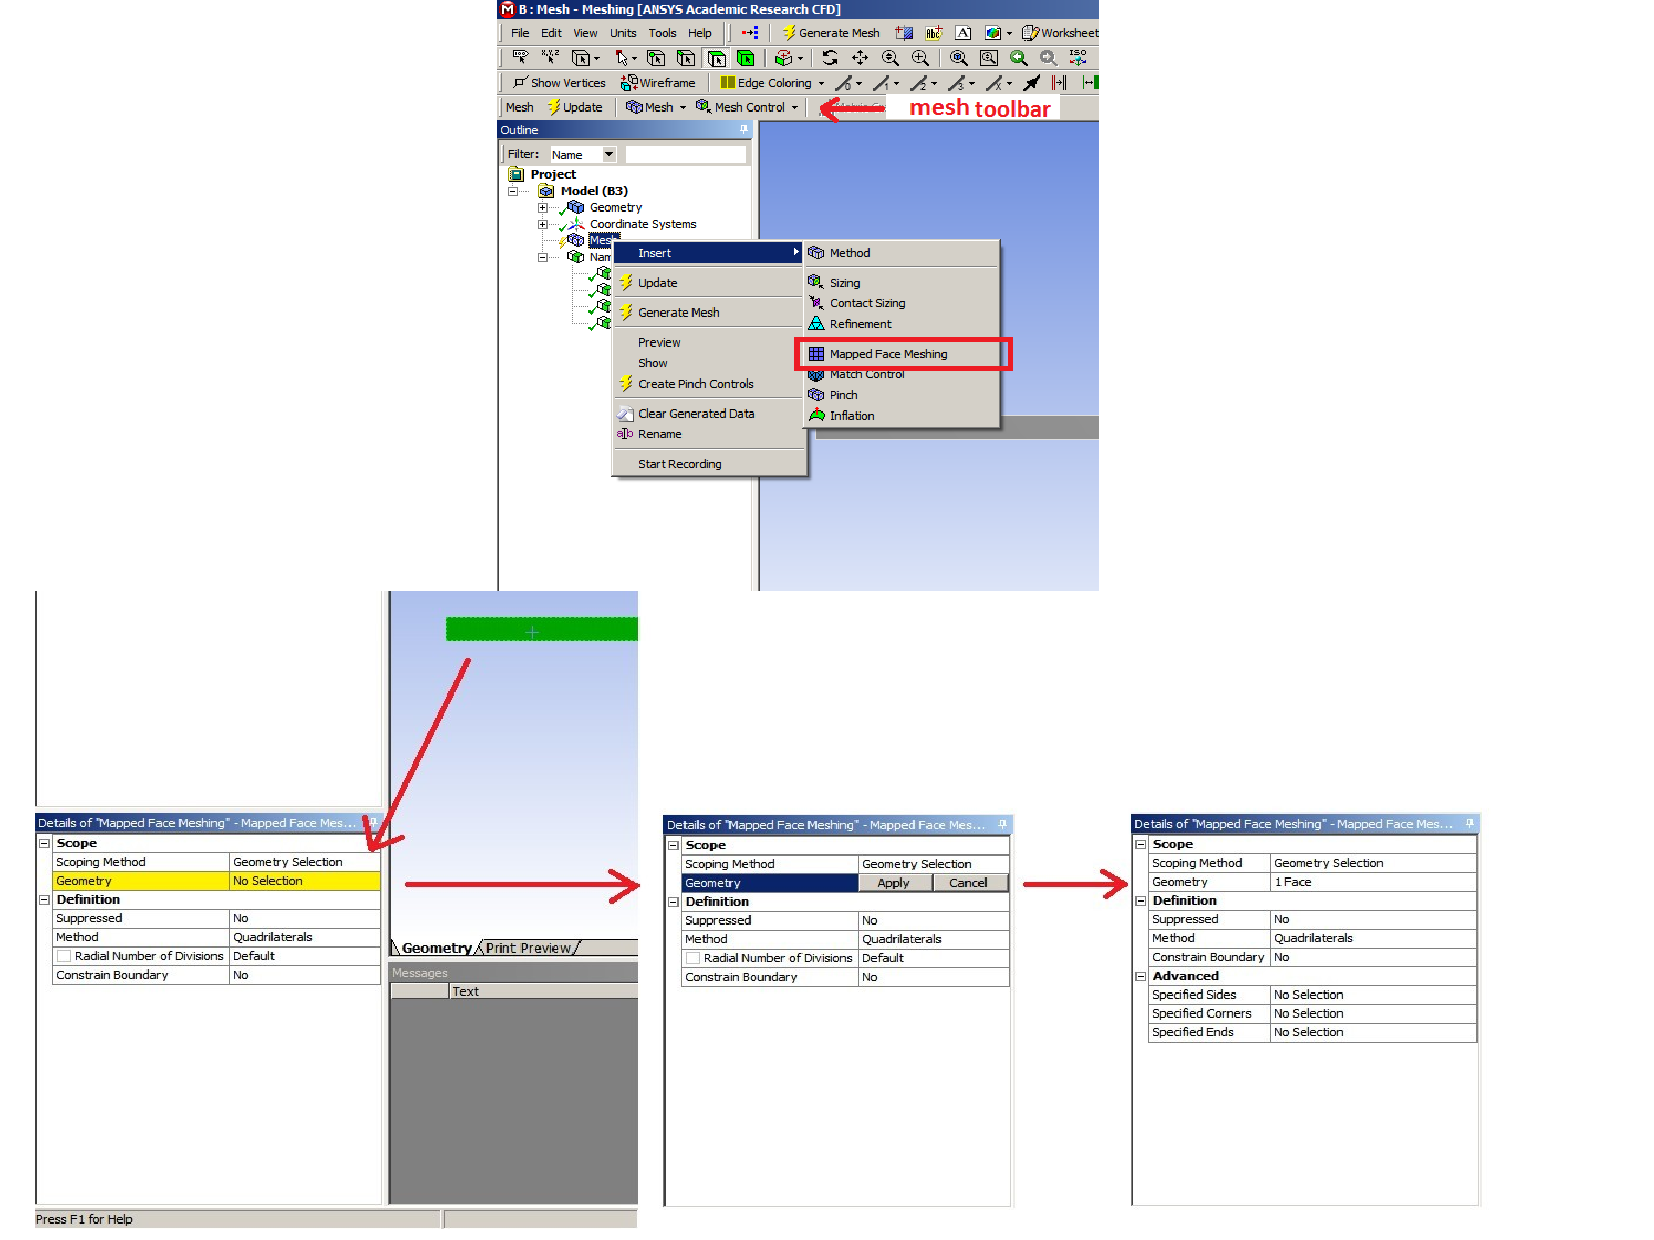
\includegraphics[width=\columnwidth, clip]{./Figs/MeshGeneration4.pdf} 
          \end{figure}}
       \end{column}
    \end{columns}
\end{frame} 

 
%%%
%%% Slide
%%%
\begin{frame}
 \frametitle{Pre-processing: Mesh Generation} 
    \begin{columns}
       \begin{column}[l]{0.5\linewidth}
          \begin{enumerate}\scriptsize\setcounter{enumi}{5}
             \item<1-> Now we need to generate the mesh:
                \begin{enumerate}[a)]\scriptsize
                   \item<2-> Right-click \blue{Mapped Face Meshing} from the \blue{Tree Outline};
                   \item<2-> Select \blue{Generate Mesh};
                   \item<2-> We just created a structured mesh
                \end{enumerate}
          \end{enumerate}
       \end{column}
       \begin{column}[l]{0.5\linewidth}
          \visible<2->{\begin{figure}
                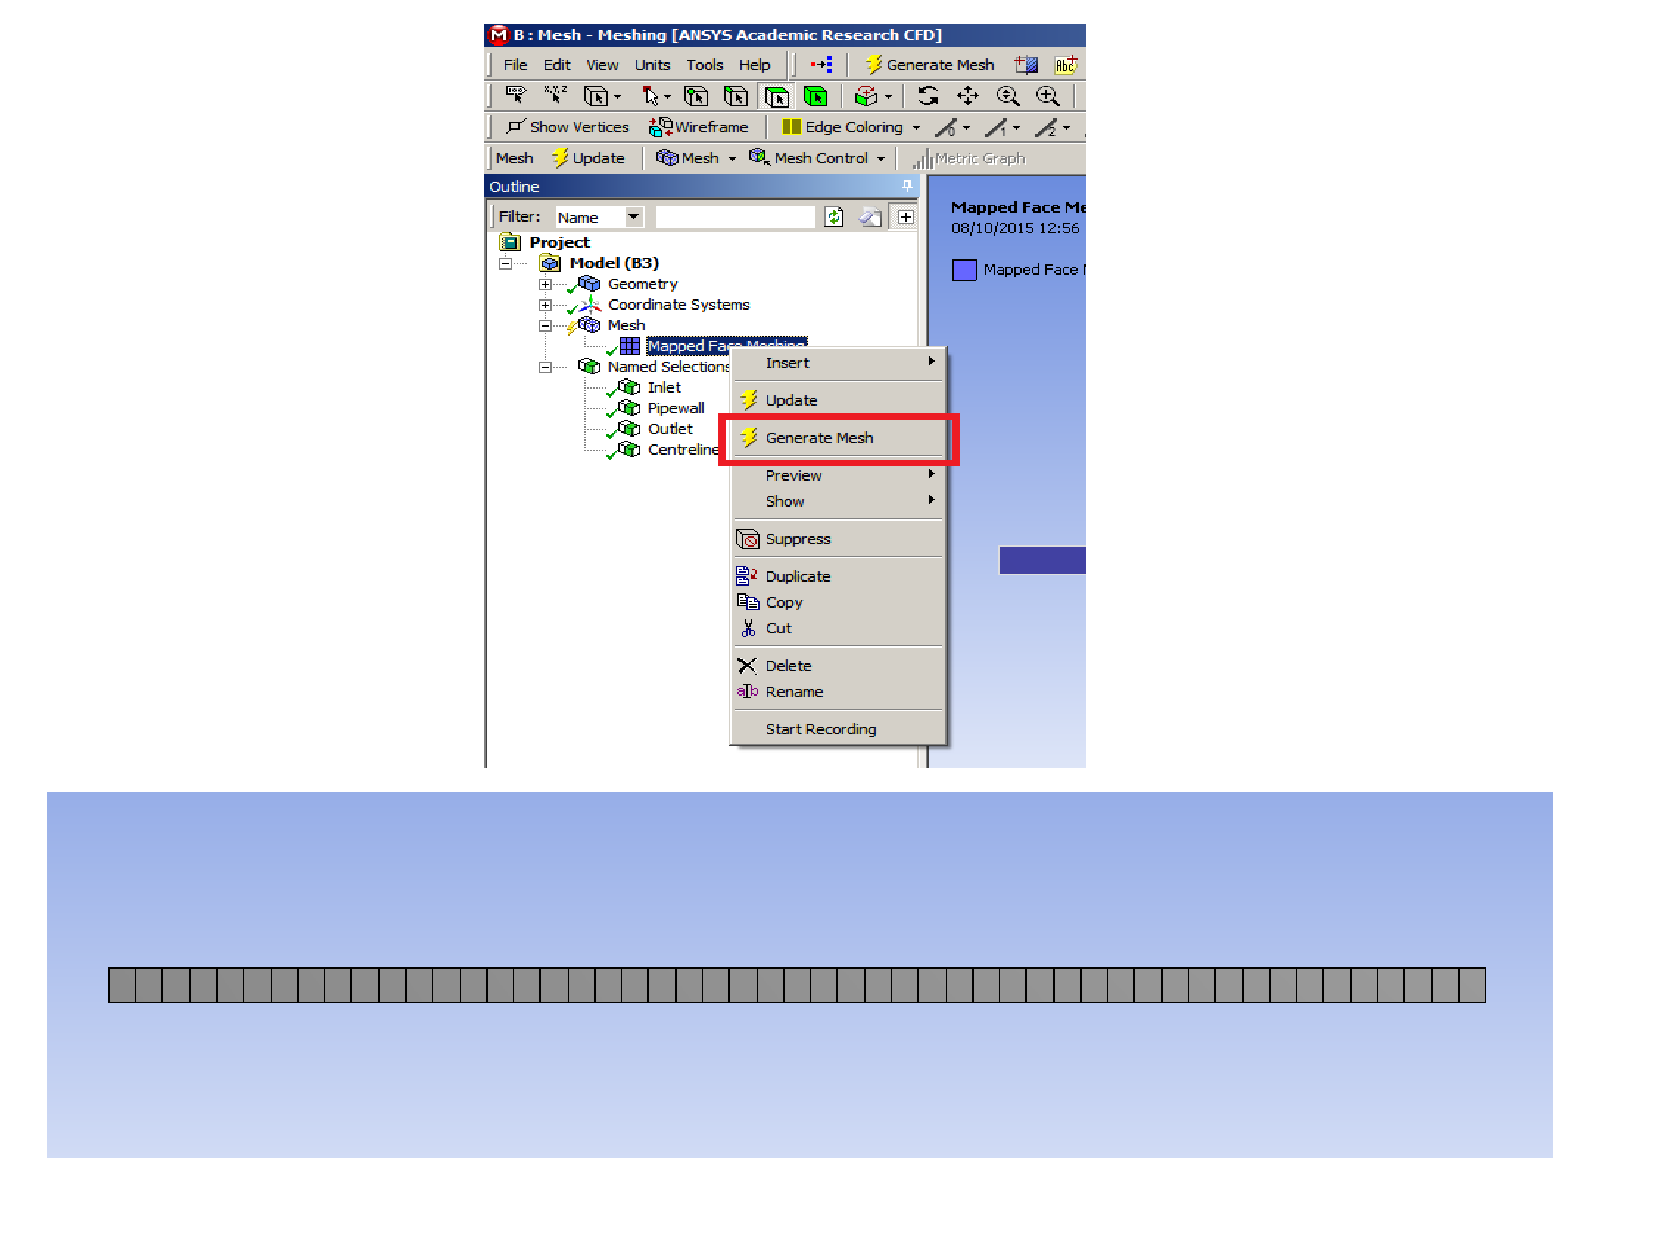
\includegraphics[width=\columnwidth, clip]{./Figs/MeshGeneration5.pdf} 
          \end{figure}}
       \end{column}
    \end{columns}
\end{frame} 

 
%%%
%%% Slide
%%%
\begin{frame}
 \frametitle{Pre-processing: Mesh Generation} 
    \begin{columns}
       \begin{column}[l]{0.5\linewidth}
          \begin{enumerate}\scriptsize\setcounter{enumi}{6}
             \item<1-> After generating a mesh that conforms with the geometry, we need to `adjust' the grid, \ie either refine it or coarse it;
             \item<2-> The default grid consists of 51 cells (remember that ANSYS Fluent is based on FVM discretisation) that be checked through \blue{Mesh} $\rightarrow$ \blue{Statistics};
             \item<3-> For this problem, we aim to refine the mesh towards 600 cells: 8 in the vertical and 75 in the horizontal;
             \item<4-> Thus, we need to adjust the \red{cell size}, \ie the number of divisions through the {\it x-} and {\it y-}directions;
                \begin{enumerate}[a)]\scriptsize
                   \item<5-> Click \blue{Mesh Control} from the \blue{Mesh Toolbar} $\Rightarrow$ \blue{Sizing};
                   \item<5-> The \blue{Edge Tool} must be selected, and with the \red{\it Ctrl-key} pressed, select the top and bottom edge of the geometry (which now should be \red{green});
                   \item<5-> Click \blue{Apply} from the \blue{Details View} and;
                   \item<5-> In this box, change \blue{Number of Divisions} to \blue{75}, \blue{Behavior} to \blue{Hard} and \blue{No Bias};
                   \item<5-> Click the \blue{Update} botton from the \blue{Mesh Toolbar};
                \end{enumerate}
          \end{enumerate}
       \end{column}
       \begin{column}[l]{0.5\linewidth}
          \visible<2->{\begin{figure}
                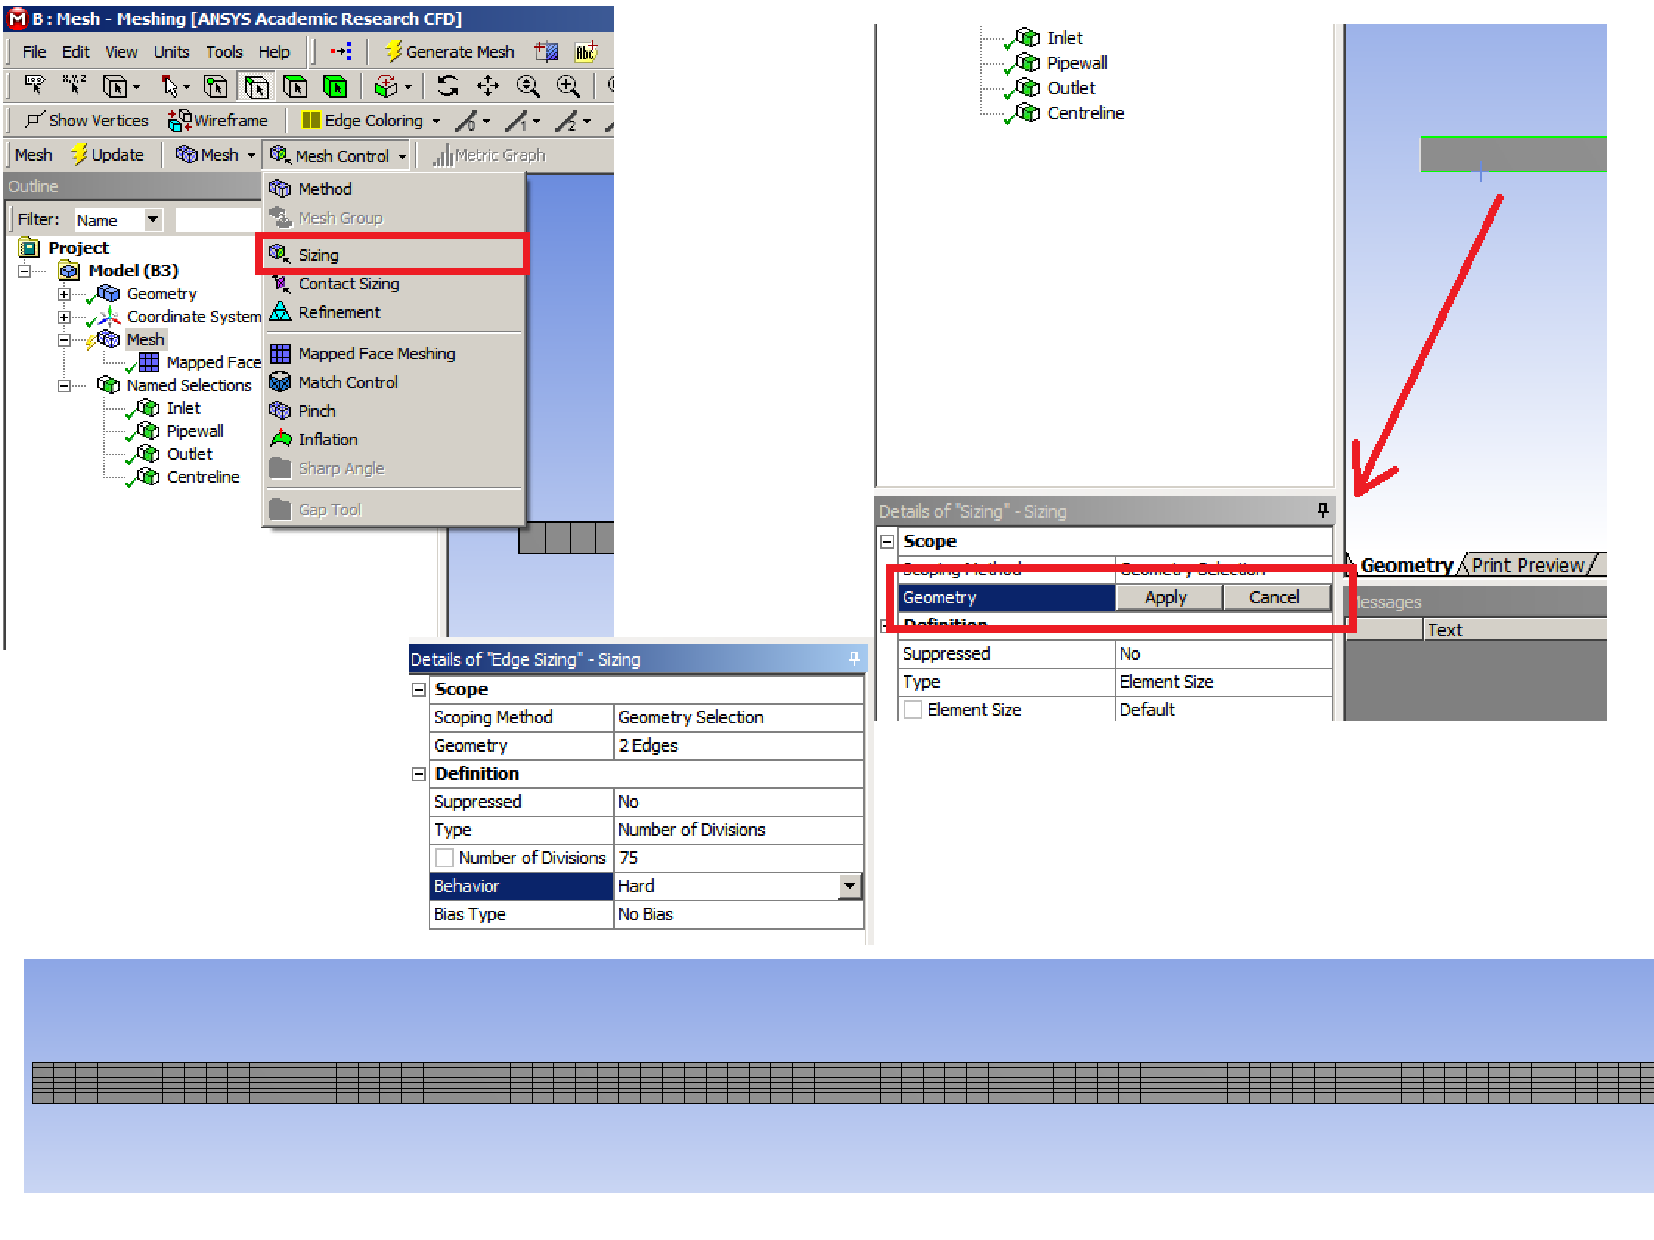
\includegraphics[width=\columnwidth, clip]{./Figs/MeshGeneration6.pdf} 
          \end{figure}}
                \begin{enumerate}[f)]\scriptsize
                   \item<6-> Repeat the procedure for the left and right boundaries with \red{8} divisions.
                \end{enumerate}
          \visible<7->{\scriptsize Save the project and close the \blue{Meshing} windows and, in the \blue{Workbench}, click \blue{Update project} and \red{save} the project once more.}
       \end{column}
    \end{columns}
\end{frame} 

 
%######################
%%%   SUBSUBSECTION
%######################
\subsubsection{Pre-Processing: Model Setup}

%%%
%%% Slide
%%%
\begin{frame}
  \frametitle{Pre-processing: Model Setup}
    \begin{columns}
        \begin{column}[l]{0.5\linewidth}
           \begin{enumerate}\scriptsize
                \item<1-> After establishing \red{Dimensionality}, \red{Geometry} and the associated \red{Mesh Grid}, we now need to set up the mathematical problem, \ie
                    \begin{enumerate}[a)]\scriptsize
                       \item<2-> Fluid problem (and associated conservative equations and field variables);
                       \item<2-> Constitutive equations (\eg equation of state for compressible fluids, turbulence submodels etc);                 
                       \item<2-> Boundary conditions (Dirichlet, Newman and/or Robin);                 
                       \item<2-> Initial conditions;                 
                       \item<2-> Thermofluid properties; 
                       \item<2-> Solution methods that will be used to solve the set of conservative and constitutive equations. 
                    \end{enumerate}
                \item<3-> In the \blue{Workbench},
                    \begin{enumerate}[i)]\scriptsize
                       \item<3-> Drag the \blue{Fluent component} into the \blue{Project Schematic};
                       \item<3-> Drag the \blue{Mesh cell} from \blue{Component Table} to the \blue{Setup Cell} of the \blue{Fluent component};
                       \item<3-> If a symbol appear close the previously generated mesh, right-click on the \blue{Mesh} and select \blue{Update};
                       \item<3-> Right-click \blue{Setup} from \blue{Fluent component} and select \blue{Refresh};
                    \end{enumerate}                    
           \end{enumerate}
        \end{column}
           \begin{column}[l]{0.5\linewidth}
               \visible<3->{\begin{center}
                   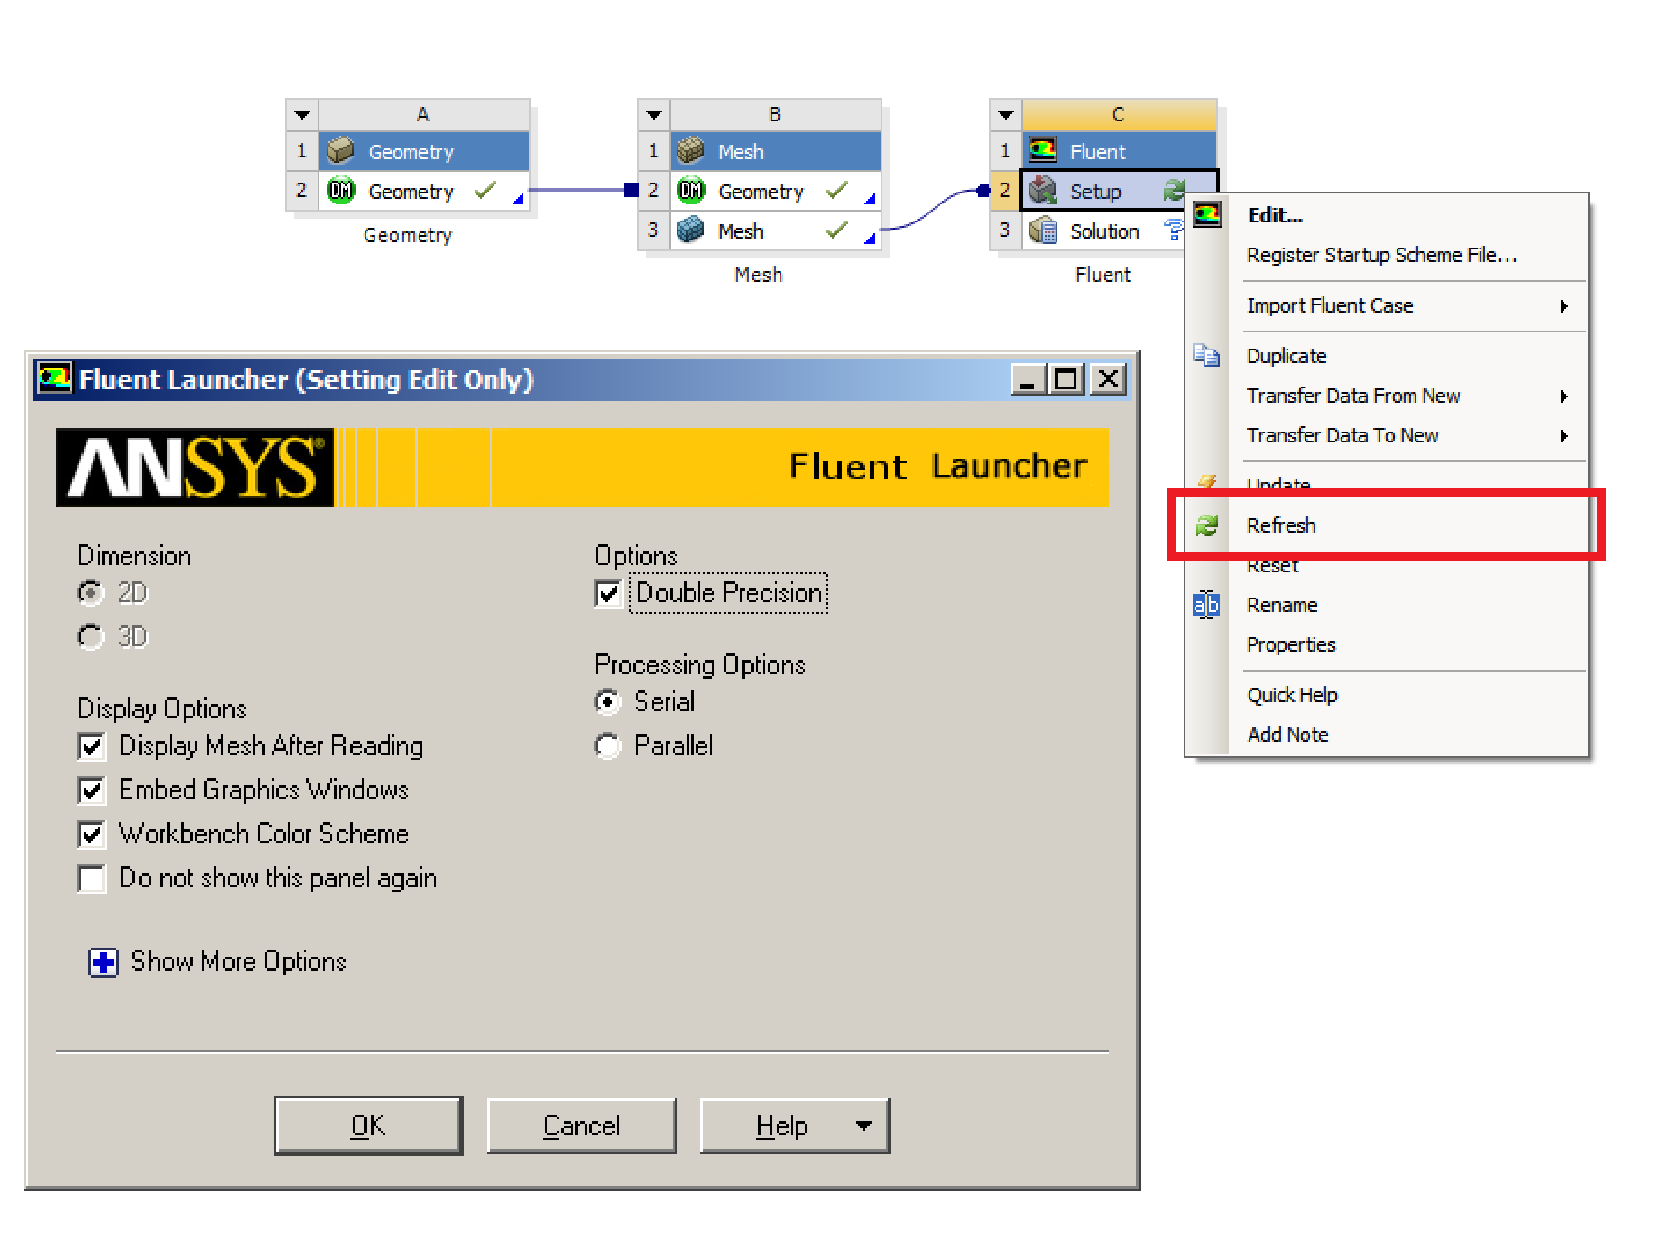
\includegraphics[width=\columnwidth, clip]{./Figs/ProblemSetup1.pdf}
               \end{center}}
               \begin{enumerate}[i)]\scriptsize\setcounter{enumi}{4}
                   \item<3-> Double-click \blue{Setup} $\Rightarrow$ \blue{Double Precision};
               \end{enumerate}
           \end{column}
    \end{columns}
\end{frame}
    

%%%
%%% Slide
%%%
\begin{frame}
  \frametitle{Pre-processing: Model Setup}
    \begin{columns}
        \begin{column}[l]{0.4\linewidth}
           \begin{enumerate}\scriptsize\setcounter{enumi}{2}
               \item<1-> Check \red{warning} and \red{error} messages in the \blue{Console};  
               \item<2-> If there are \red{warning} messages -re \red{boundary zones}, then 
                    \begin{enumerate}[i)]\scriptsize
                        \item<2-> Select \blue{Cell Zone Conditions} from the \blue{Navigation Panel} and;
                        \item<2-> From the \blue{Task Panel}, change \blue{Type} to \blue{Fluid}.
                   \end{enumerate}  
               \item<3-> Now, we need to check if the mesh is correctly imported into the \red{Fluent Solver}, and to setup the model as {\it \red{axisymmetric}},
                    \begin{enumerate}[i)]\scriptsize
                        \item<3-> Click \blue{General} from \blue{Navigation Panel} and select \blue{Axisymmetric};
                        \item<3-> In the \blue{Menu bar} select: \blue{Mesh} $\Rightarrow$ \blue{Info} $\Rightarrow$ \blue{Size};
                   \end{enumerate}  
               \item<4-> The \blue{Console} should show info -re to the mesh. 
           \end{enumerate}
        \end{column}
           \begin{column}[l]{0.6\linewidth}
               \visible<2->{\begin{center}
                   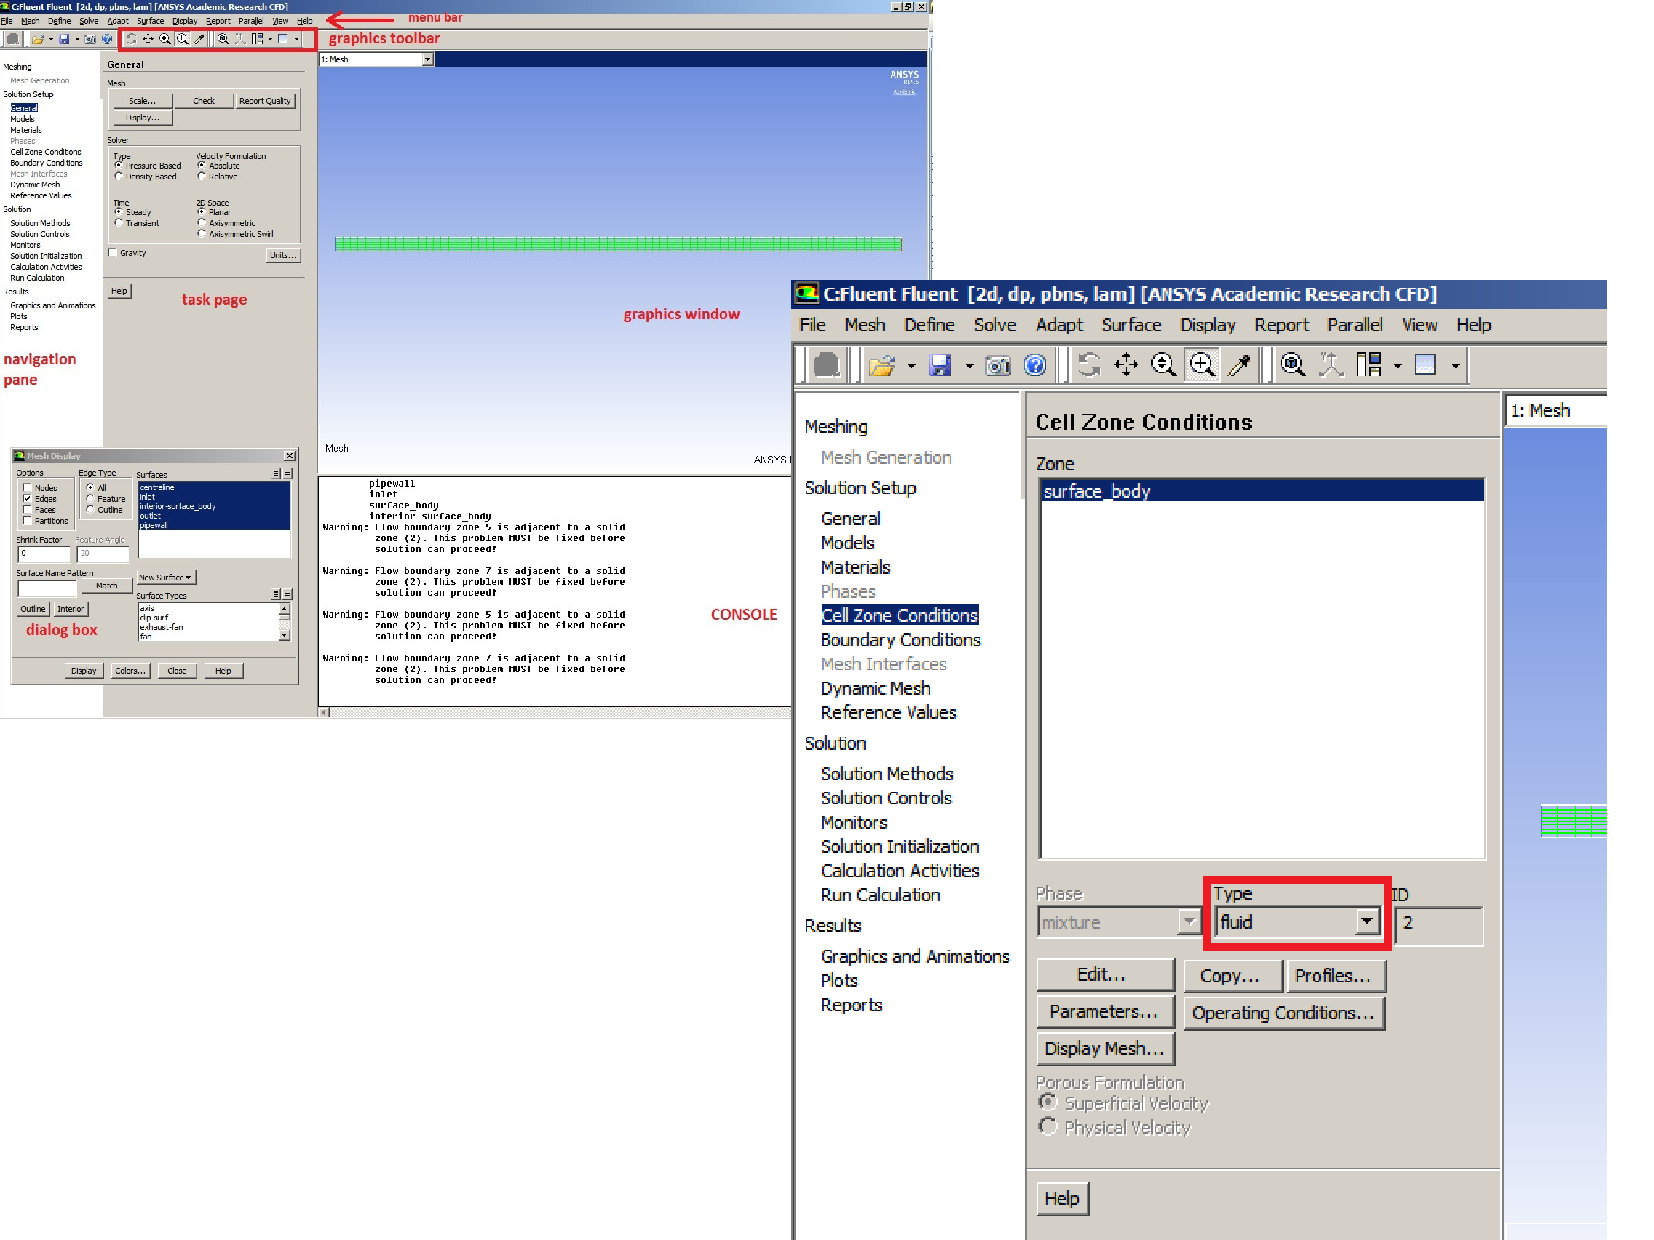
\includegraphics[width=\columnwidth, clip]{./Figs/ProblemSetup2.pdf}
               \end{center}}
           \end{column}
    \end{columns}
    \begin{center}
        \visible<4->{\begin{tabular}{c c c c c}
             \scriptsize Levels  & \scriptsize Cells &  \scriptsize Faces  & \scriptsize Nodes & \scriptsize Partitions \\
             \scriptsize   0     & \scriptsize  600  &  \scriptsize  1283  & \scriptsize 684   & \scriptsize     1     
        \end{tabular}}
    \end{center}
    \visible<4->{\begin{center}        
        \scriptsize 1 cell zone, 5 face zones.
    \end{center}}

    
\end{frame}



%%%
%%% Slide
%%%
\begin{frame}
  \frametitle{Pre-processing: Model Setup}
    \begin{columns}
        \begin{column}[l]{0.5\linewidth}
           \begin{enumerate}\scriptsize\setcounter{enumi}{6}
                \item<1-> Setup \red{Model}:
                    \begin{enumerate}[i)]\scriptsize
                       \item<1-> Select \blue{Models} from the \blue{Navigation Panel};
                       \item<1-> Select \blue{Viscous Model} and click \blue{Edit};
                       \item<1-> Select \blue{Laminar};
                       \item<1-> And ensure that \red{all} other models (\eg multiphase, energy etc) are disabled.                      
                   \end{enumerate}
                \item<2-> Setup \red{Materials}:
                    \begin{enumerate}[i)]\scriptsize
                       \item<2-> Select \blue{Materials} from the \blue{Navigation Panel};
                       \item<2-> Select \blue{Air} from the \blue{Task Page} under \blue{Materials};
                       \item<2-> Click \blue{Create/Edit};
                       \item<2-> In the \blue{Dialogue Box}, change \blue{Properties} of the fluid to the required values, \ie $\rho=$ 1.0 kg.m$^{-3}$, $\mu=$ 1.5$\times$10$^{-3}$ kg.(m.s)$^{-1}$;     
                       \item<2-> Click \blue{Change/Create} to close the window.                
                   \end{enumerate}                   
           \end{enumerate}
        \end{column}
           \begin{column}[l]{0.5\linewidth}
               \visible<2->{\begin{center}
                   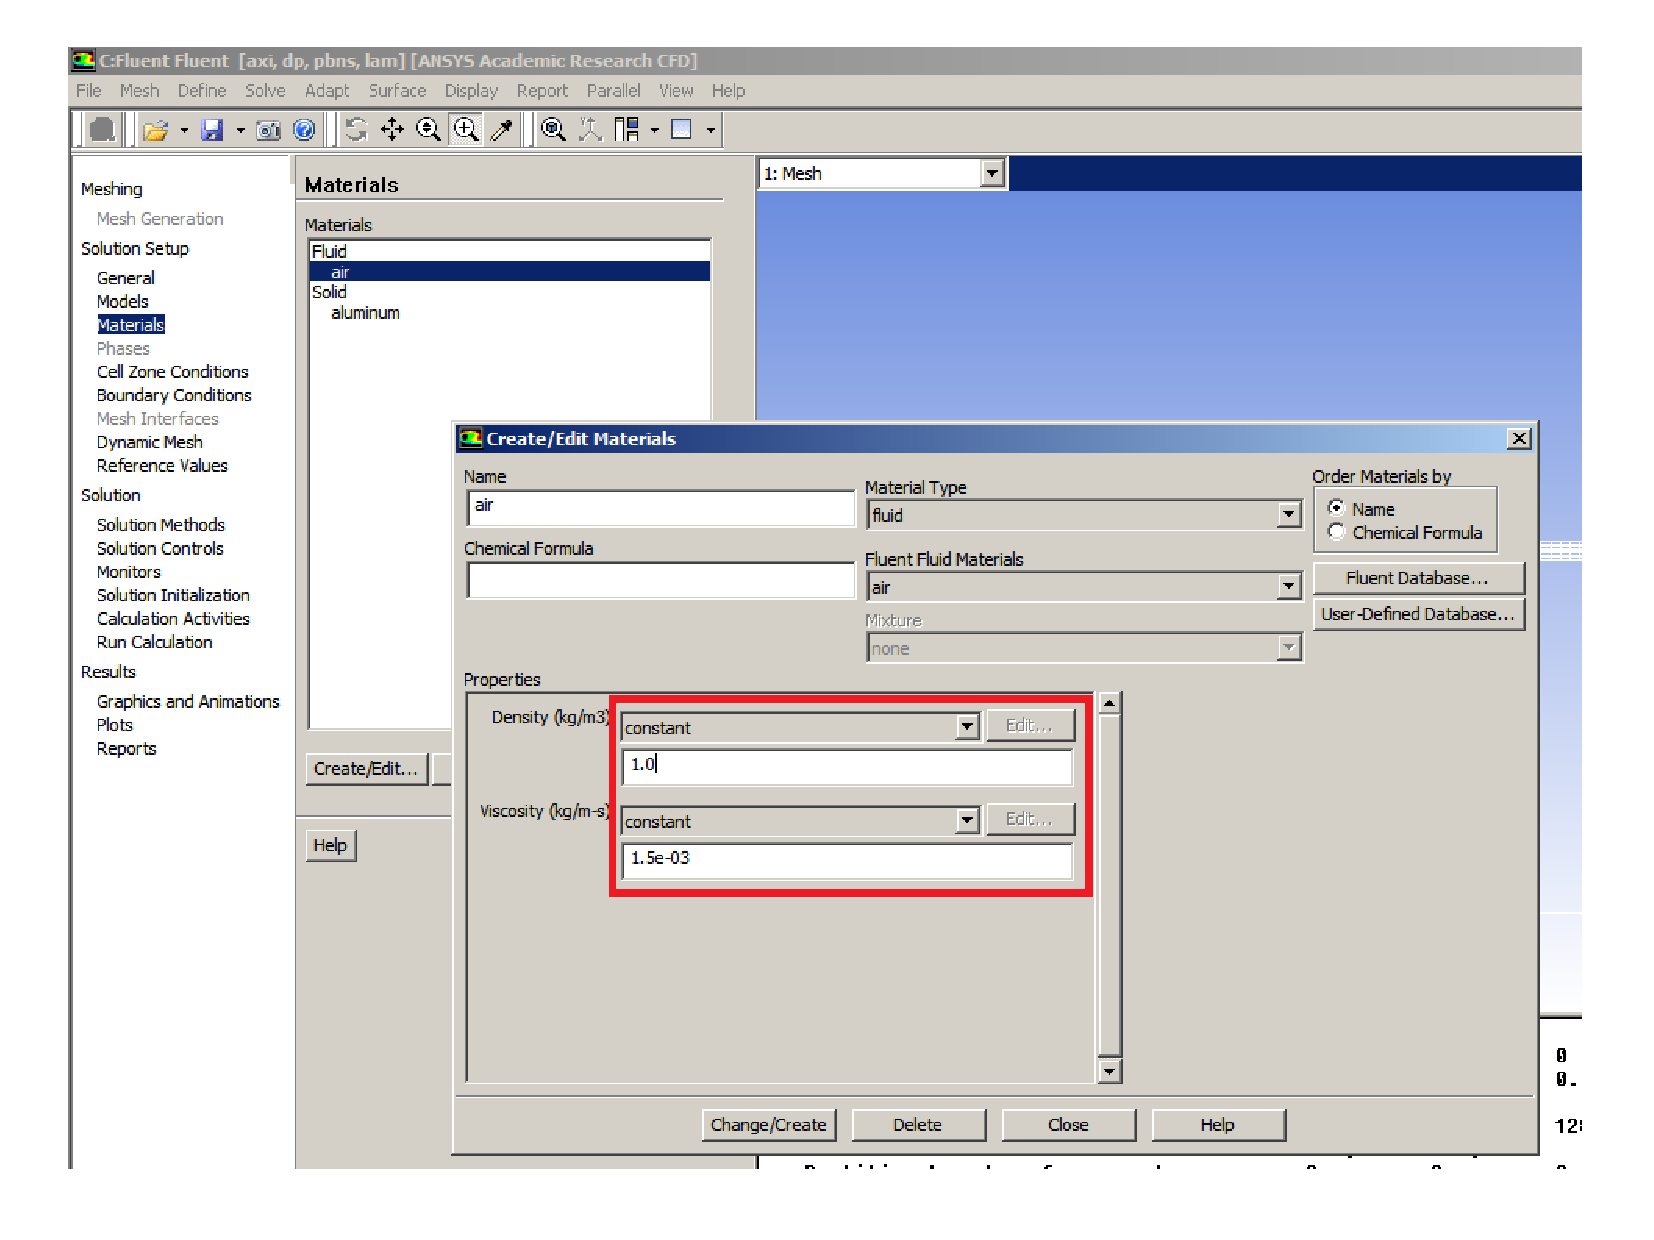
\includegraphics[width=\columnwidth, clip]{./Figs/ProblemSetup3.pdf}
               \end{center}}
           \end{column}
    \end{columns}
\end{frame}



%%%
%%% Slide
%%%
\begin{frame}
  \frametitle{Pre-processing: Model Setup}
    \begin{columns}
        \begin{column}[l]{0.5\linewidth}
           \begin{enumerate}\scriptsize\setcounter{enumi}{8}
                \item<1-> During the \red{mesh setup}, we defined the \red{boundary lines (Inlet, Outlet, Pipewall and Centreline)}, now we should set up the properties of these lines, 
                \item<2-> For the \red{Inlet BC}:
                    \begin{enumerate}[i)]\scriptsize
                       \item<2-> Select \blue{Boundary Condition} from the \blue{Navigation Panel}, and select \blue{Inlet} from the \blue{Task Page};
                       \item<2-> Click \blue{Edit} and the \blue{Velocity Inlet dialog Panel} will appear;
                       \item<2-> Set \blue{Velocity Specification Method} to \blue{Components};
                       \item<2-> Set \blue{Axial Velocity} to \blue{1 m.s$^{-1}$}; 
                    \end{enumerate}
                \item<3-> For the \red{Outlet BC}
                    \begin{enumerate}[i)]\scriptsize
                       \item<3-> Select \blue{Outlet} from the \blue{Task Page};
                       \item<3-> Select \blue{Type} $\Rightarrow$ \blue{Pressure-Outlet};
                       \item<2-> No further changes are needed since the gauge pressure by default is set to \blue{0 Pa};
                    \end{enumerate}
                \item<4-> For the \red{Pipewall BC}
                    \begin{enumerate}[i)]\scriptsize
                       \item<4-> Select \blue{Pipewall} from the \blue{Task Page};
                       \item<4-> Select \blue{Type} $\Rightarrow$ \blue{Wall};
                    \end{enumerate}
           \end{enumerate}
        \end{column}
           \begin{column}[l]{0.5\linewidth}
               \visible<2->{\begin{center}
                   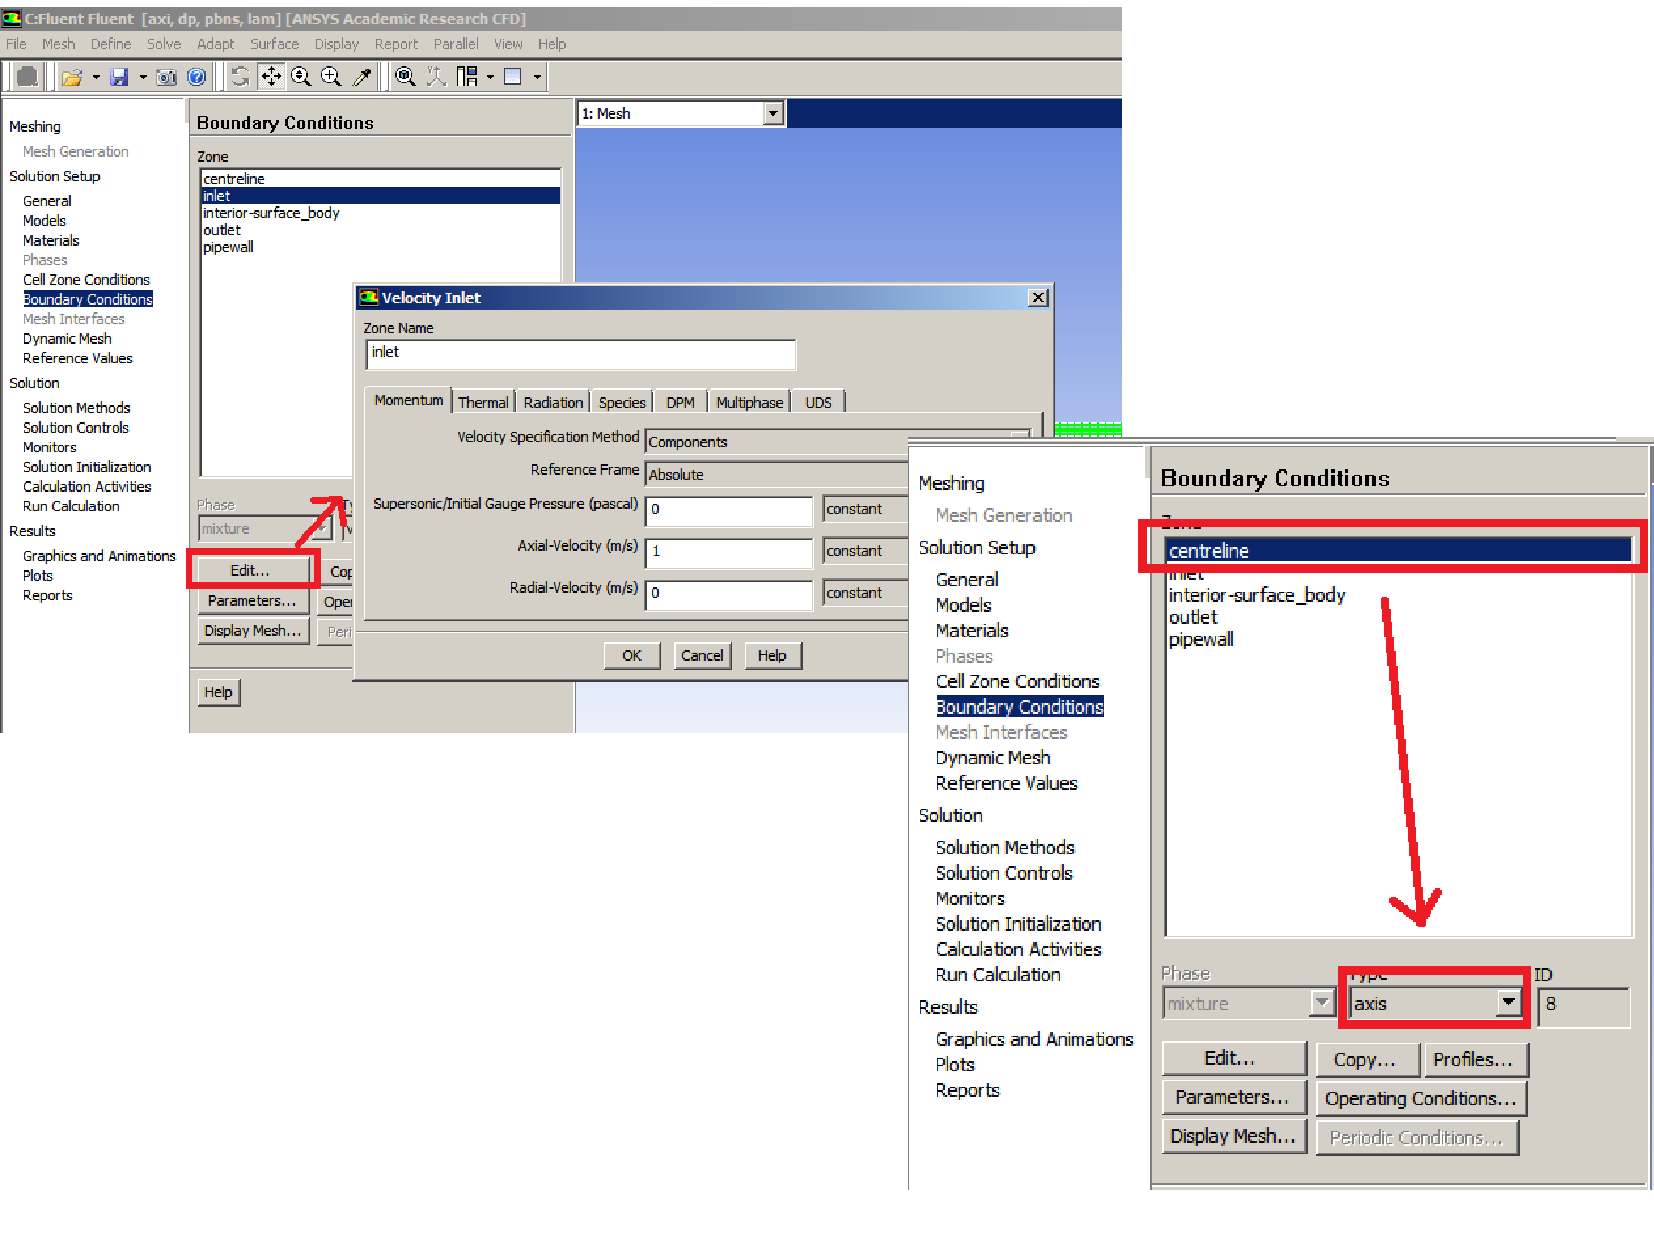
\includegraphics[width=\columnwidth, clip]{./Figs/ProblemSetup4.pdf}
               \end{center}}
               \begin{enumerate}\scriptsize\setcounter{enumi}{12}
                   \item<5-> For the \red{Centreline BC}:
                       \begin{enumerate}[i)]\scriptsize
                          \item<5-> Select \blue{Centreline} from the \blue{Task Page};
                          \item<5-> Select \blue{Type} $\Rightarrow$ \blue{Axis};
                       \end{enumerate}
               \end{enumerate}
           \end{column}
    \end{columns}
\end{frame}




%%%
%%% Slide
%%%
\begin{frame}
  \frametitle{Pre-processing: Model Setup}
    \begin{columns}
        \begin{column}[l]{0.5\linewidth}
           \begin{enumerate}\scriptsize\setcounter{enumi}{13}
                \item<1-> Now that we setup the \red{physical} and \red{mathematical} problem, we need to setup the numerical schemes that Fluent will use to discretise and solve the problem;
                \item<2-> For this problem, we will use the 2$^{\text{nd}}$-order discretisation to solve the momentum equation:
                    \begin{enumerate}[i)]\scriptsize
                        \item<2-> Select \blue{Solution Methods} from the \blue{Navigation Panel};
                        \item<2-> Select \blue{Scheme} $\Rightarrow$ \blue{SIMPLE};
                        \item<2-> For \blue{Spatial Discretisation}:
                             \begin{enumerate}[(a)]\scriptsize
                                       \item<2-> \blue{Gradient} $\Rightarrow$ \blue{Least Squares Cell Based};
                                       \item<2-> \blue{Pressure} $\Rightarrow$ \blue{Standard};
                                       \item<2-> \blue{Momentum} $\Rightarrow$ \blue{Second-Order Upwind}.
                             \end{enumerate}
                    \end{enumerate}
                \item<3-> In the \blue{Solution Controls} box we can establish {\it relaxation factors} that will be used by the \red{Solver};
                \item<3-> Select \blue{Solution Controls} from the \blue{Navigation Panel} and use the following relaxation factors:
                    \begin{enumerate}[i)]\scriptsize
                        \item<3-> \blue{Pressure} $\Rightarrow$ \blue{0.3};
                        \item<3-> \blue{Density} $\Rightarrow$ \blue{1.0};
                        \item<3-> \blue{Body Forces} $\Rightarrow$ \blue{1.0};
                        \item<3-> \blue{PressureMomentum} $\Rightarrow$ \blue{0.7};
                    \end{enumerate}
           \end{enumerate}
        \end{column}
           \begin{column}[l]{0.5\linewidth}
               \visible<2->{\begin{center}
                   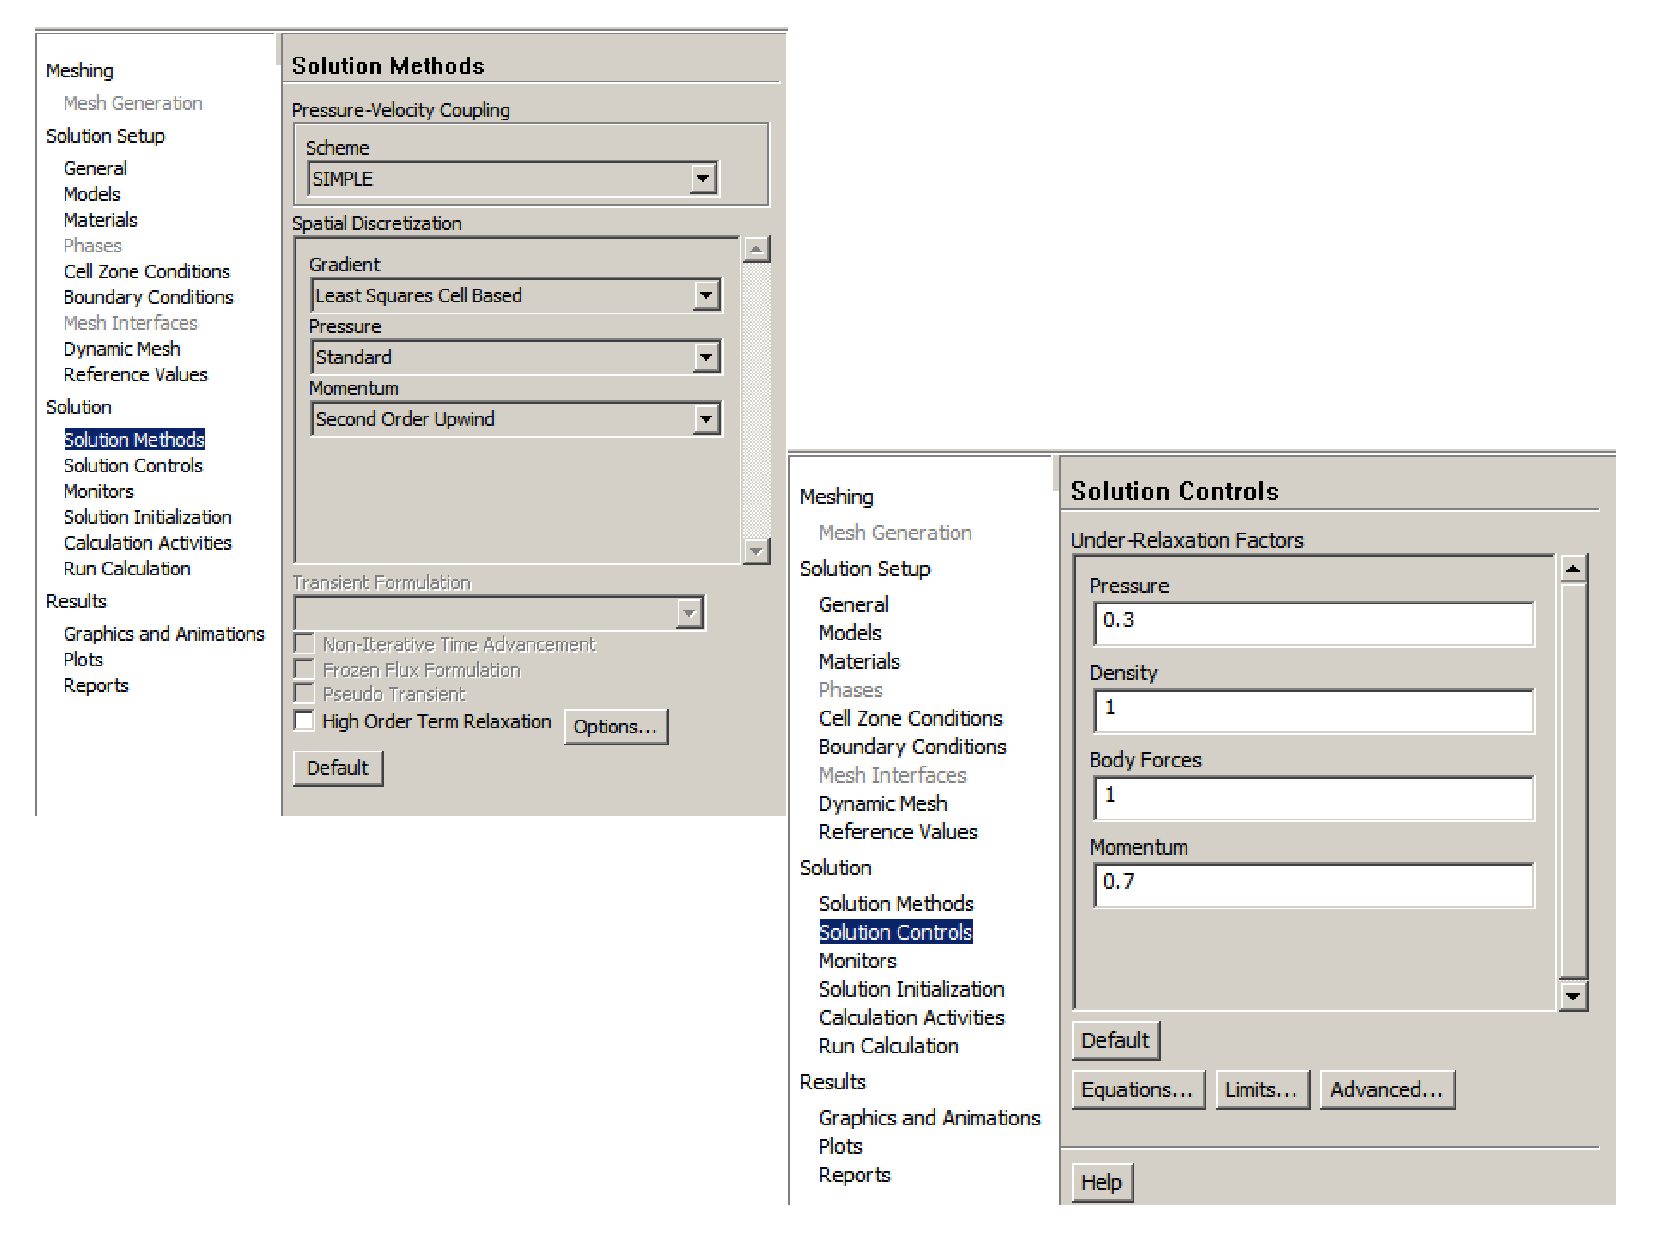
\includegraphics[width=\columnwidth, clip]{./Figs/ProblemSetup5.pdf}
               \end{center}}
           \end{column}
    \end{columns}
\end{frame}


%%%
%%% Slide
%%%
\begin{frame}
  \frametitle{Pre-processing: Model Setup}
    \begin{columns}
        \begin{column}[l]{0.5\linewidth}
           \begin{enumerate}\scriptsize\setcounter{enumi}{17}
               \item<1-> As the {\it Fluent Solver} seeks the solution for the set of PDEs representing the physical problem, it requires residuals that makes the solution acceptable.
               \item<1-> Also, we may want to monitor and control of the solution and to extract diagnostic fields to assess the temporary and final solutions;  
                    \begin{enumerate}[i)]\scriptsize
                       \item<2-> Click \blue{Monitor} from the \blue{Navigation Panel} and select \blue{Residuals} from the \blue{Task Page};
                       \item<2-> Select \blue{Residuals -- Print, Plot} from the \blue{Residuals, Statistics and Force Monitors} and;
                       \item<2-> Click \blue{Edit} and set all 3 \blue{Absolute Convergence Criteria} to \blue{1.0$\times$10$^{-6}$}
                    \end{enumerate}
                    \visible<2->{The monitors provide an overall view of the iteration convergence of the variables at all nodes and cells after every iteration.}
               \item<3-> We can monitor a specific variable in the course of the simulation, \eg force on a wall section or pressure at a specific location (this is the equivalent of installing a sensor in a physical experiment!);
           \end{enumerate}
           
        \end{column}
           \begin{column}[l]{0.5\linewidth}
               \visible<2->{\begin{center}
                   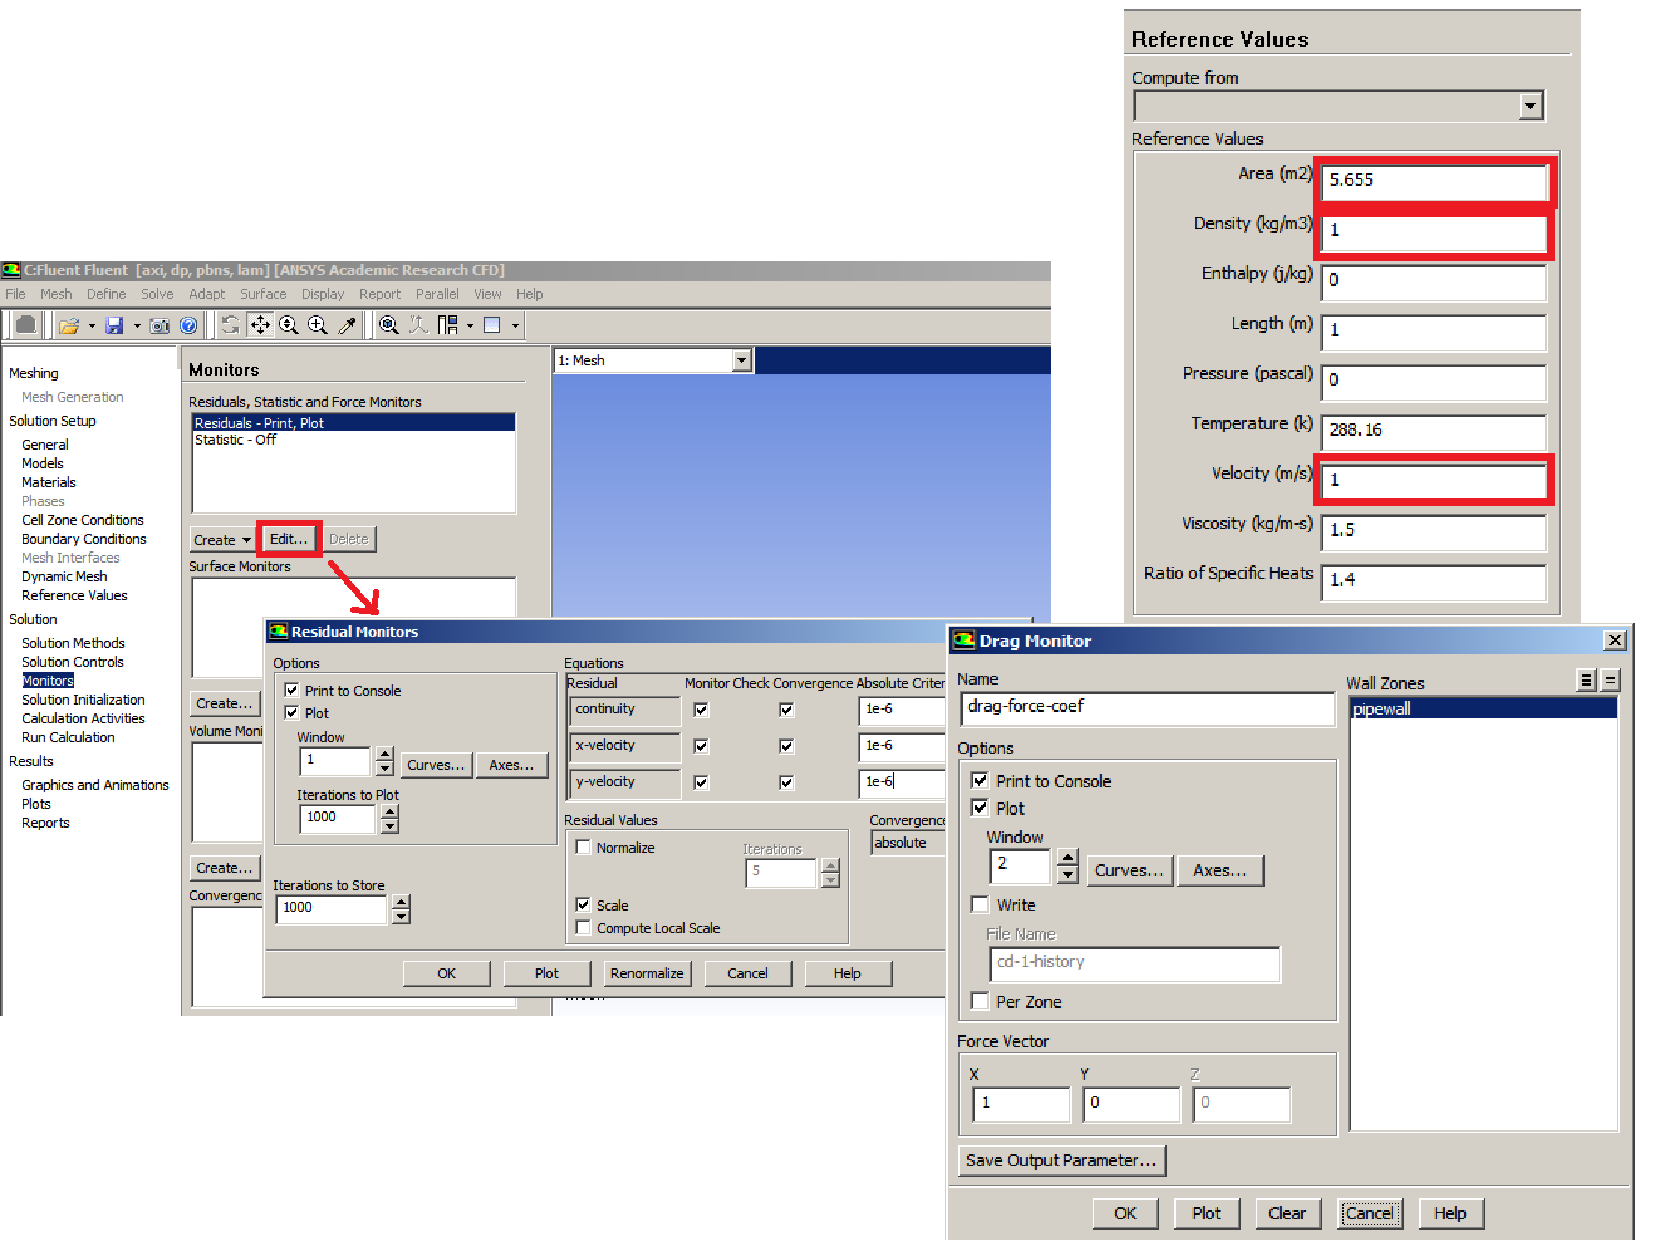
\includegraphics[width=\columnwidth, clip]{./Figs/ProblemSetup6.pdf}
               \end{center}}
           \end{column}
    \end{columns}
\end{frame}

%%%
%%% Slide
%%%
\begin{frame}
  \frametitle{Pre-processing: Model Setup}
    \begin{columns}
        \begin{column}[l]{0.5\linewidth}
           \begin{enumerate}\scriptsize\setcounter{enumi}{20}
                \item<1-> In this example, we will monitor the \red{drag coefficient on the pipe wall},
                    \begin{enumerate}[i)]\scriptsize
                       \item<1-> Click \blue{Create} in the \blue{Task Page} under \blue{Residuals, Statistics and Force Monitors};
                       \item<1-> Select \blue{Drag} and give the \blue{Monitor} a name;
                       \item<1-> Select \blue{Pipewall} from \blue{Wall Zones} and tick \blue{Print} to \blue{Console} and \blue{Plot} boxes under \blue{Options}.
                    \end{enumerate}
                \item<2-> Note that Fluent calculates the drag coefficient with respect to user-defined reference values for the density, velocity and area:
                      \begin{displaymath}\scriptsize
                          C_{D} = \frc{F_{D}}{0.5\rho_{\text{ref}}V^{2}_{\text{ref}}A_{\text{ref}}} = \frc{\int\overline{\tau}_{w}\overline{a}dA}{0.5\rho_{\text{ref}}V^{2}_{\text{ref}}A_{\text{ref}}}
                      \end{displaymath}
                      \visible<2->{The drag force $F_{D}$ is calculated in Fluent by integrating the wall shear stress $\overline{\tau}_{w}$ over the wall area, here $\overline{a}$ indicates the direction in which the force is acting.}
                \item<3-> Now, in the \blue{Reference Values} box from the \blue{Navigation Panel}, specify \blue{Density} and \blue{Velocity} values (Fig.~\ref{SchematicsPipe}) and set the \blue{Area} equal to the area of the pipe $\left(A_{\text{ref}}=2\pi r L\right)$;    
           \end{enumerate}
        \end{column}
           \begin{column}[l]{0.5\linewidth}
               \visible<1->{\begin{center}
                   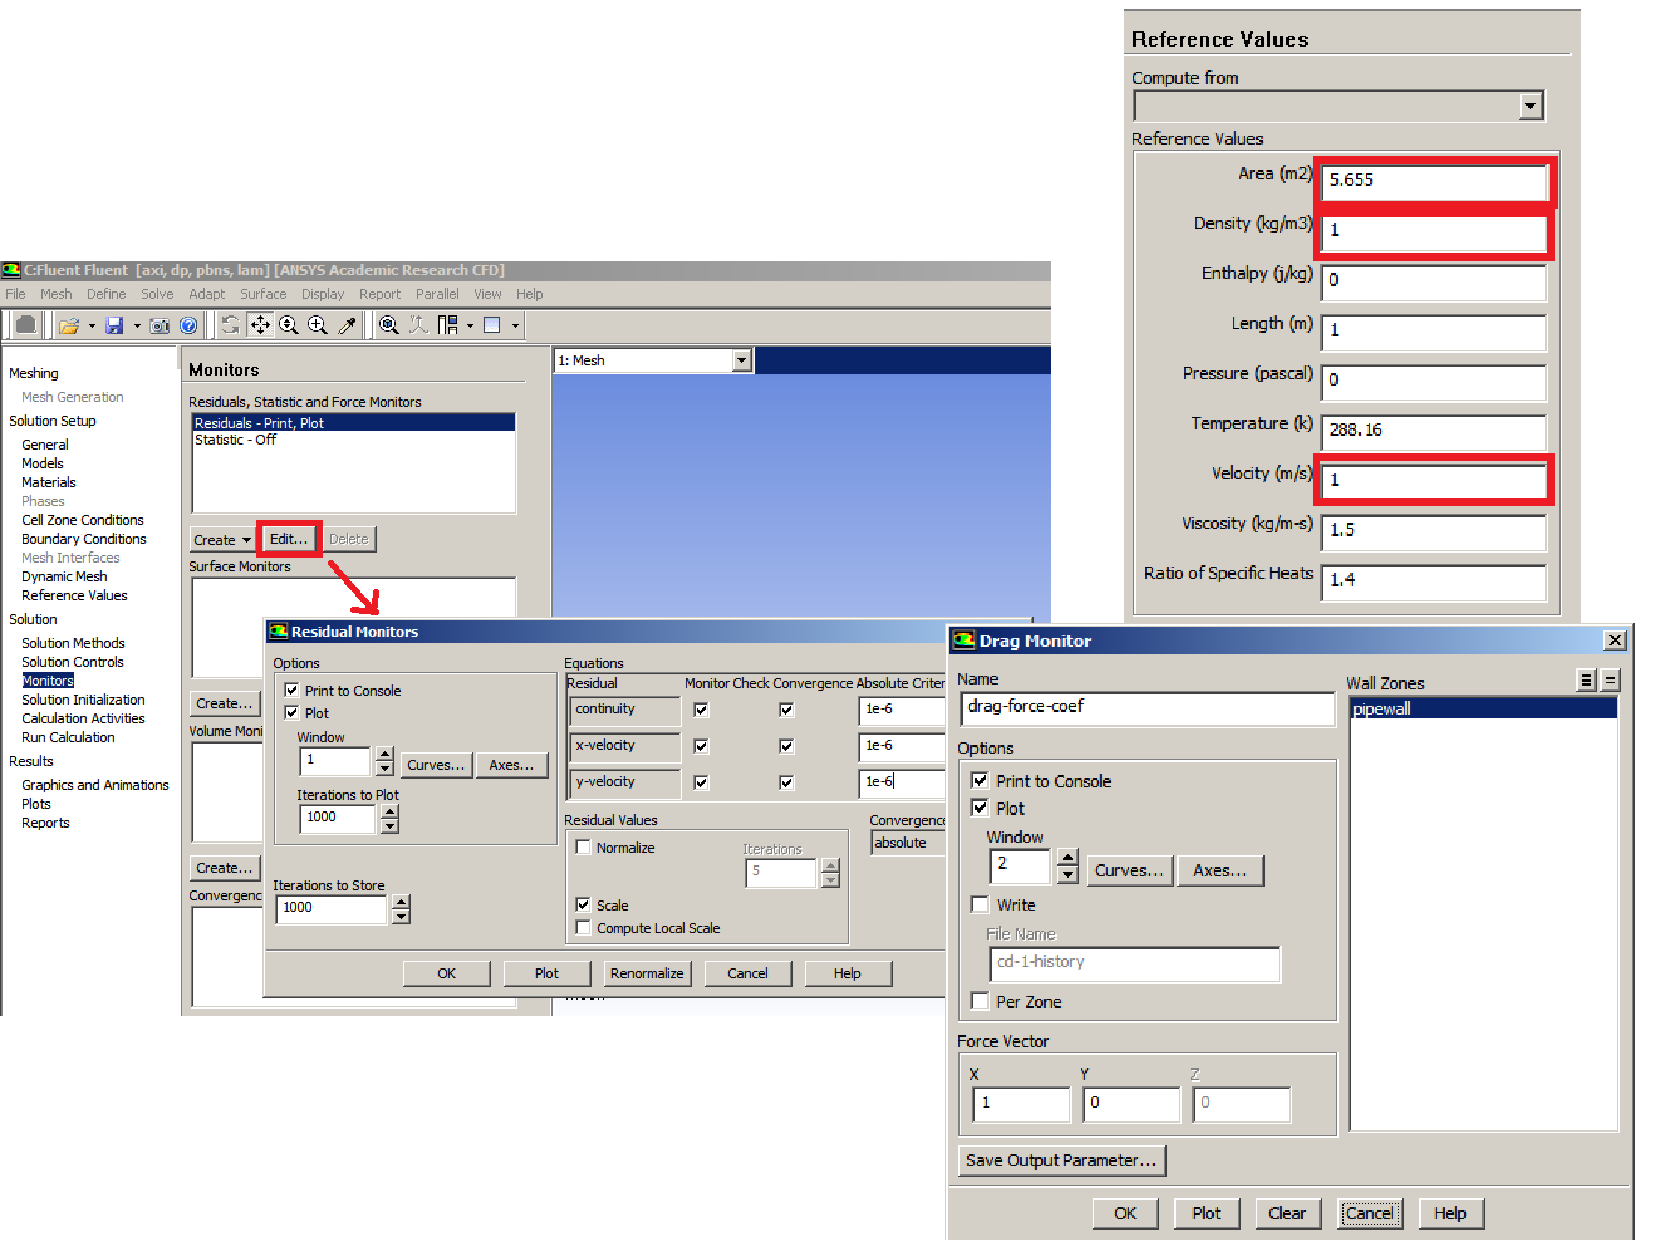
\includegraphics[width=\columnwidth, clip]{./Figs/ProblemSetup6.pdf}
               \end{center}}
           \end{column}
    \end{columns}
\end{frame}

%%%
%%% Slide
%%%
\begin{frame}
  \frametitle{Pre-processing: Model Setup}
    \begin{columns}
        \begin{column}[l]{0.5\linewidth}
           \begin{enumerate}\scriptsize\setcounter{enumi}{23}
                \item<1-> The last stage in the \red{pre-processing} before running the simulation is to \red{initialise} the problem, \ie set up \red{Initial Conditions}.
                \item<1-> For this example, initial pressure and velocity (axial and radial components) are prescribed;
                    \begin{enumerate}[i)]\scriptsize
                       \item<2-> Select \b;lue{Solution Initialisation} from the \blue{Navigation Panel};
                       \item<2-> Select \blue{Standard Initialisation} and choose \blue{Inlet} and;
                       \begin{enumerate}[(a)]\scriptsize
                          \item<2-> \blue{Gauge Pressure} $\Rightarrow$ \blue{0.0 Pa}; 
                          \item<2-> \blue{Axial Velocity} $\Rightarrow$ \blue{1.0 m.s$^{-1}$}; 
                          \item<2-> \blue{Radial Velocity} $\Rightarrow$ \blue{0.0 m.s$^{-1}$}; 
                       \end{enumerate}
                       \item<2-> Press \blue{Initialise}.
                    \end{enumerate}                    
           \end{enumerate}
        \end{column}
           \begin{column}[l]{0.5\linewidth}
               \visible<2->{\begin{center}
                   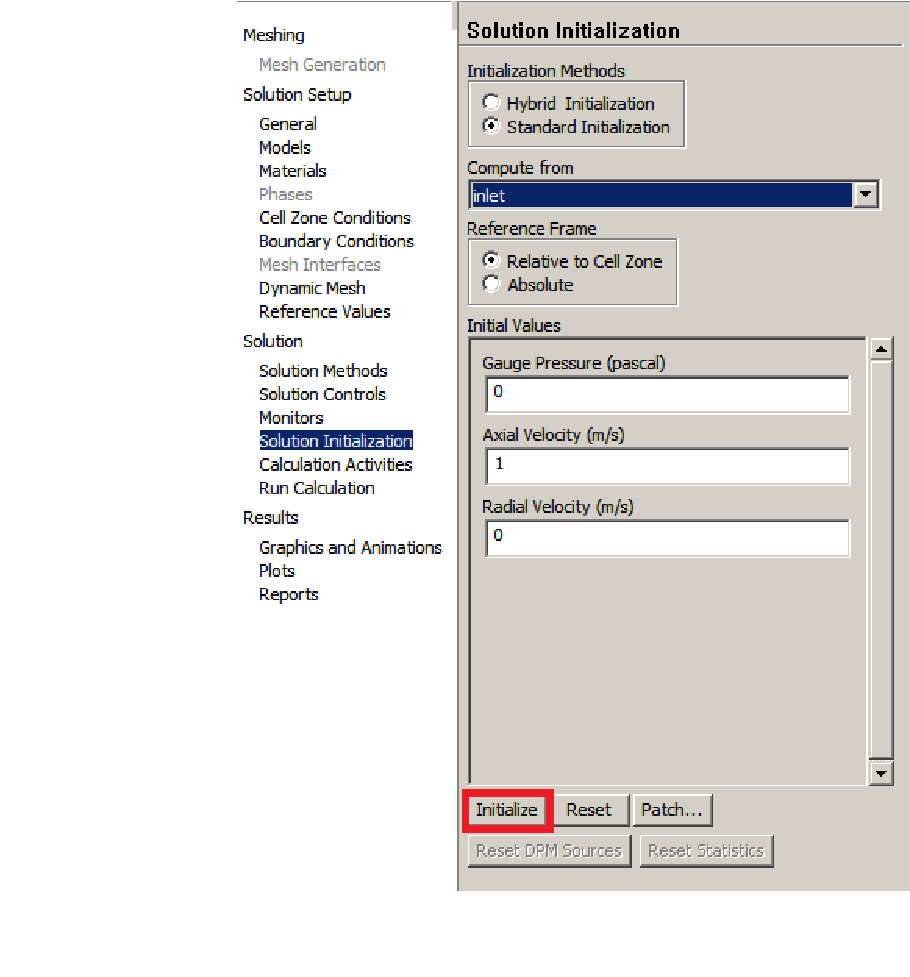
\includegraphics[width=\columnwidth, clip]{./Figs/ProblemSetup7.pdf}
               \end{center}}
           \end{column}
    \end{columns}
\end{frame}

\end{document}
